\documentclass[12pt]{nmsuth01}
%If your system does not have a latex package ``pkg'', for example,
 %attempting to run latex on the file will produce an error report
 %reading something like ``Latex error:  File pkg.sty not found.''
%
%Your system should have the latex symbol package.  If not comment out 
 %the next line by placing a percent sign % at the beginning of the line.
\usepackage{latexsym}
%Your system may not have the American Mathematical Society packages
 %for mathematics and theorem formatting.  If not, comment out the
 %next line.  If you comment out the next line, you should also
 %comment out all the theorem formatting commands, and you should not
 %try to process the part of the document called chp1a.tex.  Commment
 %out the line below calling for \input{chp1a}.
\usepackage{amsmath,amsthm,mathtools}
%For bra-ket notation
\usepackage{physics}
\DeclarePairedDelimiterX\phys[3]{\langle}{\rangle}{#1 \delimsize\vert\mathopen{} #2 \delimsize\vert\mathopen{} #3}
\newcommand*\Vector[1]{\boldsymbol{#1}}
%For slash notation
\usepackage{slashed}
%For tables
\usepackage{tabularx}
%Your system may not have the xypic drawing package.  If not, comment
 %out the next line.  If you comment out the next line, you should
 %also not try to process chp1a.tex.  
\usepackage[all]{xy}
%Your system should have the graphicx package for included graphics.
 %If not, or, if you have no graphics to include, comment out the next 
 %line.  If you commment out the next line, then you should not try to 
 %process the part of the document called graphics.tex.  Comment out
 %the line below calling for \section{SAMPLE TEXT WITH GRAPHICS} \label{graphics}
%This file illustrates how include in your thesis graphical
 %output.
%The next line produces an indented paragraph to start the document
 %unit.  The LaTeX defaults start most units without indentations.
\hspace{\parindent}
This is sample text with graphics.
\begin{figure}[h]
  \centering
  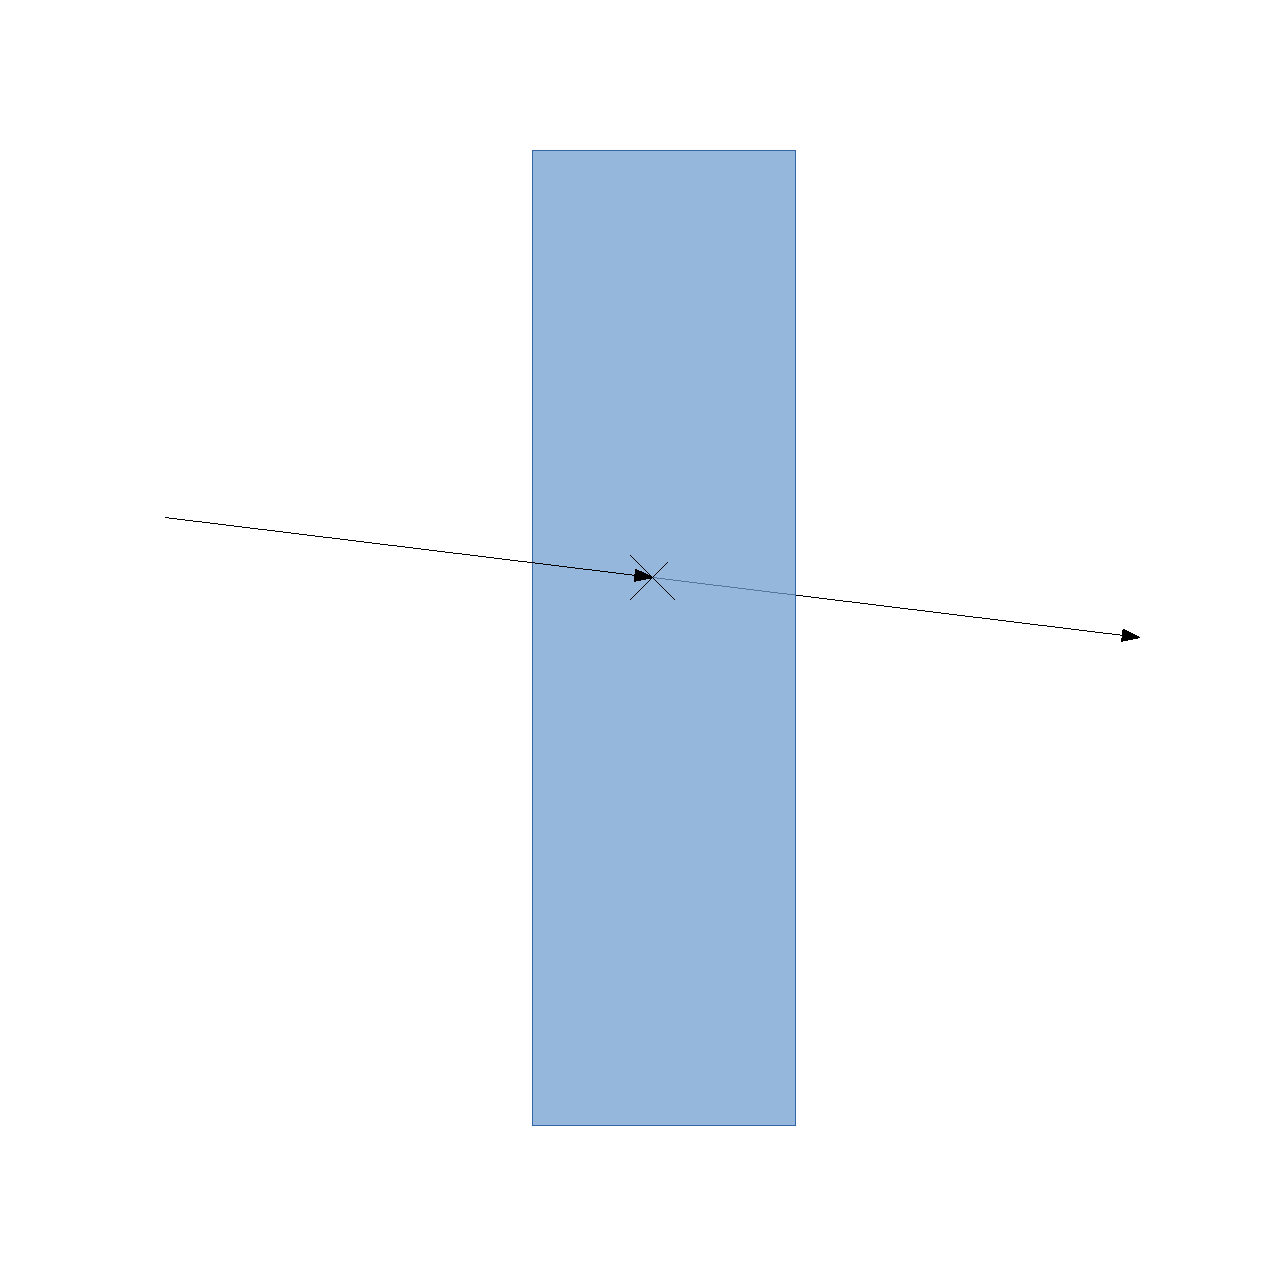
\includegraphics[angle=-90,width=4in]{figures/bz.pdf}
  \caption{This is an inserted EPS graphic}
  \label{fig:mygraph1}
\end{figure}
Sample ref of \ref{fig:mygraph1} 

\begin{figure}[t]
 \centering
  \includegraphics[angle=-90, width=4in]{figures/E734eta.pdf}  
    \caption{This is another inserted PDF graphic}
    \label{fig:mygraph2}
\end{figure}
%This is the end of the file graphics.tex


\usepackage{graphicx}
\usepackage{subcaption}
\usepackage{float}
\usepackage{placeins}
%The next settings give the correct margins for an NMSU Ph.D. thesis.
\setlength{\evensidemargin}{0.5in}
\setlength{\oddsidemargin}{0.5in}
\setlength{\textwidth}{5.75in}
\setlength{\topmargin}{-0.25in}
\setlength{\textheight}{8.25in}
%
%
% Theorem Formatting Commands.
\theoremstyle{plain}
\newtheorem{lemma}{Lemma}[section]
\newtheorem{prop}{Proposition}[section]
\newtheorem{theorem}{Theorem}[section]
\newtheorem{cor}{Corollary}[section]
%\newtheorem*{nametheorem}{Theorem}[section]
\theoremstyle{definition}
\newtheorem{defn}{Definition}[section]
\newtheorem{example}{Example}[section]
\theoremstyle{remark}
\newtheorem*{rem}{Remark}
\newtheorem*{convention*}{Convention}
%
% Miscellaneous Special Capitals
\newcommand{\bZ}{{\mathbf Z}}
\newcommand{\bQ}{{\mathbf Q}}
\newcommand{\bR}{{\mathbf R}}
\newcommand{\cC}{{\mathcal C}}
% 
%Miscellaneous symbols
%\newcommand{\op}{{\rm \oplus}}
\newcommand{\id}{\rm id}
%
%Miscellaneous Greek letters
\newcommand{\eps}{\ensuremath{\epsilon}}
\newcommand{\ga}{\ensuremath{\gamma}}
%
%Miscellaneous operators
\DeclareMathOperator{\Coker}{Coker}
\DeclareMathOperator{\Tor}{Tor}
\DeclareMathOperator{\Ext}{Ext}
\DeclareMathOperator{\Maps}{Maps}
\DeclareMathOperator{\Hom}{Hom}
\DeclareMathOperator{\Aut}{Aut}
\DeclareMathOperator{\Sin}{Sin}
\DeclareMathOperator{\Tot}{Tot}
\DeclareMathOperator{\im}{im}
%
%Prepare for  double spacing
%\renewcommand{\baselinestretch}{1.5}
\newlength{\singlespace}
\setlength{\singlespace}{\baselineskip}
\newlength{\doublespace}
\setlength{\doublespace}{2.0\baselineskip}
%
\begin{document}
%Use the next line to obtain double spacing for the main body of the document
\setlength{\baselineskip}{\doublespace}
%Comment out the preceding line and uncomment the next line containing
 %a \setlength command to obtain single spacing for the main body of 
 %the document.
%\setlength{\baselineskip}{\singlespace}
%
%Why do you care about this option?
%There are two answers.  One is that it takes less paper to print a
 %preliminary draft of the thesis.  The second is that singlespacing
 %makes the structural units of the document more apparent.  Single
 %spacing makes it easy to identify definitions, lemmas, theorems, and 
 %so on, and it makes apparent such problems as a paragraph that is
 %running too long. On the other hand, the double spacing is good for 
 %checking for typographical errors in a manuscript.  Note that a 
 %document printed in singlespacing and doublespacing formats will 
 %have its problems with page and line breaks in different locations.  
%
%The title page, approval page, dedication page, acknowledgment page,
 %vita page, abstract page, and pages listing tables and figures (if
 %there are any) all carry roman numerals.
\pagenumbering{roman}
\pagestyle{empty}
%This file makes a title page for a Ph.D. thesis.
\thispagestyle{empty}
\renewcommand{\baselinestretch}{2}
\begin{center}
NEUTRAL CURRENT ELASTIC SCATTERING \\ AND THE STRANGE SPIN STRUCTURE OF THE PROTON
\vspace{0.1in}
BY\\
\vspace{0.1in}
KATHERINE WOODRUFF
\end{center}
\vspace{1.0in}
\begin{center}
A dissertation submitted to the Graduate School\\
\vspace{0.1in}
in partial fulfillment of the requirements\\
\vspace{0.1in}
for the degree \\
\vspace{0.1in}
Doctor of Philosophy
\end{center}
\vfill
\begin{center}
Major Subject: Physics
\end{center}
\vspace{1.0in}
\begin{center}
New Mexico State University\\
\vspace{0.1in}
Las Cruces New Mexico\\
\vspace{0.1in}
November 2018
\end{center}
\newpage
%This is the end of the title page.

\pagestyle{plain}
%This file makes the approval page for a Ph.D. thesis at NMSU.  It
 %must be replaced when a permanent Dean of the Graduate School is named.
\noindent
``Neutral Current Elastic Scattering and the Strange Spin Structure of the Proton,'' 
a dissertation prepared by
Katherine Woodruff 
in partial fulfillment of the requirements for the degree, 
Doctor of Philosophy,
has been approved and accepted by the following:

\setlength{\baselineskip}{\singlespace}
\vspace{0.1in}
\begin{flushleft}
\hrulefill
\newline
Dr. Luis Cifuentes
\newline
Dean of the Graduate School
\vspace{0.5in}

\hrulefill
\newline
Vassili Papavassiliou
\newline
Chair of the Examining Committee
\vspace{0.5in}

\hrulefill
\newline
Date
\vspace{0.5in}
\newline
Committee in charge:
\end{flushleft}

\setlength{\baselineskip}{\doublespace}
Dr. Vassili Papavassiliou, Chair

Dr. Stephen Pate

Dr. Igor Vasiliev

Dr. Steven Stochaj

\newpage
%This is the end of the approval page.

%
%%This file makes a dedication page.
\begin{center}
DEDICATION
\end{center}
%The next blank line is needed to have the dedication text
 %appropriately indented.

I dedicate this work to my mom, dad, sister, bill.

\newpage
%This is the end of the dedication page.

%
%%This file makes a page for acknowledgments.
\begin{center}
ACKNOWLEDGMENTS
\end{center}
%The next blank line is needed to have the dedication text
 %appropriately indented.

I would like to thank my advisor, ...

\newpage
%This is the end of the page for acknowledgments.

%
%%This file makes a vita page in the required two column format.
\begin{center}
            VITA
\end{center}
\begin{flushleft}
\begin{tabular}{ll}
2006-2009        &  A.S., Linn-Benton Community College, Albany, Oregon
\\
& \\
2009-2012        &  B.S., University of Oregon, Eugene, Oregon
\\
& \\
2012-2015        &  M.S., New Mexico State University, Las Cruces, New Mexico
\end{tabular}
\end{flushleft}
\vspace{0.1in}
\begin{center}PUBLICATIONS
\end{center}
  C. Adams \textit{at al.}, "A Deep Neural Network for Pixel-Level Electromagnetic Particle Identification in the MicroBooNE Liquid Argon Time Projection Chamber”," \textit{Submitted to: Phys. Rev. D}, 2018. \\
  C. Adams \textit{at al.}, "Comparison of Muon-Neutrino-Argon Multiplicity Distributions Observed by MicroBooNE to GENIE Model Predictions," \textit{Submitted to: Phys. Rev. D}, 2018. \\
  C. Adams \textit{at al.}, "Ionization Electron Signal Processing in Single Phase LAr TPCs II: Data/Simulation Comparison and Performance in MicroBooNE," \textit{JINST}, vol. 13, no. 07, p. P07007, 2018. \\
  C. Adams \textit{at al.}, "Ionization Electron Signal Processing in Single Phase LAr TPCs I: Algorithm Description and Quantitative Evaluation with MicroBooNE Simulation," \textit{JINST}, vol. 13, no. 07, p. P07006, 2018. \\
  R. Acciarri \textit{at al.}, "The Pandora Multi-Algorithm Approach to Automated Pattern Recognition of Cosmic Ray Muon and Neutrino Events in the MicroBooNE Detector," \textit{Eur. Phys. J.}, vol. C78, p. 82, 2018. \\
  R. Acciarri \textit{at al.}, "Measurement of Cosmic Ray Reconstruction Efficiencies in the MicroBooNE LAr TPC Using a Small External Cosmic Ray Counter," \textit{JINST}, vol. 12, no. 12, p. P12030, 2017. \\
  R. Acciarri \textit{at al.}, "Noise Characterization and Filtering in the MicroBooNE Liquid Argon TPC," \textit{JINST}, vol. 12, no. 08, p. P08003, 2017. \\
  R. Acciarri \textit{at al.}, "Michel Electron Reconstruction Using Cosmic-Ray Data from the MicroBooNE LArTPC," \textit{JINST}, vol. 12, no. 09, p. P09014, 2017. \\
  P. Abratenko \textit{at al.}, "Determination of Muon Momentum in the MicroBooNE LArTPC Using an Improved Model of Multiple Coulomb Scattering," \textit{JINST}, vol. 12, no. 10, p. P10010, 2017. \\
  R. Acciarri \textit{at al.}, "Convolutional Neural Networks Applied to Neutrino Events in a Liquid Argon Time Projection Chamber," \textit{JINST}, vol. 12, no. 03, p. P03011, 2017. \\
   R. Acciarri \textit{et al.}, "Design and Construction of the MicroBooNE Detector," \textit{JINST}, vol. 12, no. 02, p. P02017, 2017. \\
\begin{center}
FIELD OF STUDY
\end{center}
\begin{flushleft}
Major Field: Experimental Particle Physics
\end{flushleft}

\newpage
%This is the end of the vita page.

%
%This file makes an abstract for a Ph.D. thesis.
\begin{center}
ABSTRACT
\end{center}
\vspace{0.3in}
\begin{center}
THESIS\\ TITLE
\\
BY
\\
KATHERINE WOODRUFF
\end{center}
\vspace{0.3in}
\begin{center}
Doctor of Philosophy

New Mexico State University

Las Cruces, New Mexico, 201?

Dr. Vassili Papavassiliou, Chair
\end{center}
\vspace{0.3in}
%The next line produces an indented paragraph to start the document
 %unit.  The LaTeX defaults start most units without indentations.
\hspace{\parindent}
This is the abstract.

\newpage
%This is the end of the abstract.

\tableofcontents
%If you have tables you will use the next three lines to create a list 
 %of tables following the table of contents page.  If you have no
 %tables in your document, then you comment out the next three lines
 %by placing a percent sign (%) at the beginning of each line.  You
 %may also delete the next three lines if they are not needed.
\newpage
\listoftables
\addcontentsline{toc}{section}{LIST OF TABLES}
%If you have figures you will use the next three lines to create a
 %list of figures following the table of contents page (and the list
 %of tables, if there is one).  If you have no list of figures, then
 %you comment out the next three lines by placing a percent sign (%)
 %at the beginning of the line.  You may also delete the next three
 %lines if they are not needed.
\newpage
\listoffigures
\addcontentsline{toc}{section}{LIST OF FIGURES}
%The next two lines are essentially the start of the main body of the
 %thesis.  You go to a new page, start numbering in arabic numerals,
 %and input the introduction. 
\newpage
\pagenumbering{arabic}
%
\section{Introduction} \label{sec:intro}
%The next line produces an indented paragraph to start the document
 %unit.  The LaTeX defaults start most units without indentations.
\hspace{\parindent}

%%%%%%%%%%%%%%%%%%%%%%%%%%%%%%%%%%%%%%%%%%%%%%%%%%%%%%%%%%%
% Standard Model
%%%%%%%%%%%%%%%%%%%%%%%%%%%%%%%%%%%%%%%%%%%%%%%%%%%%%%%%%%%
\subsection{The Standard Model}\label{sec:standardmodel}

Quarks, nucleons, neutrinos. Electromagnetic and weak forces.


%%%%%%%%%%%%%%%%%%%%%%%%%%%%%%%%%%%%%%%%%%%%%%%%%%%%%%%%%%%
% Spin Structure of Nucleons
%%%%%%%%%%%%%%%%%%%%%%%%%%%%%%%%%%%%%%%%%%%%%%%%%%%%%%%%%%%
\subsection{The Spin Structure of Nucleons} \label{sec:nuctheory}

  \subsubsection{Spin Structure Functions}
  In inclusive lepton-nucleon deep inelastic scattering (DIS), it is useful to
  parameterize the scattering cross section in terms of nucleon structure
  functions $F_1(x)$, $F_2(x)$, $g_1(x)$, and $g_2(x)$. In the QCD parton
  model~\cite{Feynman:1969wa}, $x$ is the fraction of the nucleon's momentum
  carried by the quarks, and $g_1$ and $g_2$, the spin structure functions,
  parameterize the polarized DIS cross section~\cite{Thomas:2001kw}.

  The $g_1$ spin structure function can be written as a combination of the spin
  contribution from each of the quark flavors~\cite{Bass:2007zzb},
  \begin{equation*}
    g_1(x) \frac{1}{2}\sum_q e_q^2 \Delta q(x) \,,
  \end{equation*}
  where $q$ is the quark flavor ($q = u,d,s$), $e_q$ is the electric charge of
  the quark, and $\Delta q$ is the contribution from the quark spin
  contribution to the nucleon spin,
  \begin{equation*}
    \Delta q(x) = \big(q^{\uparrow} + \bar{q}^{\uparrow}\big)(x) 
      - \big(q^{\downarrow} + \bar{q}^{\downarrow}\big)(x) \,.
  \end{equation*}
  Here $q^{\uparrow}(x)$ \big($q^{\downarrow}(x)$\big) is the probability of
  finding a quark with momentum fraction $x$ with its spin polarized in the
  (opposite) direction of the nucleon's spin, and $\bar{q}^{\uparrow}(x)$
  \big($\bar{q}^{\downarrow}(x)$\big) is the probability of finding an
  antiquark with momentum fraction $x$ with its spin polarized in the
  (opposite) direction of the nucleon's spin. Integrating over the quark spin
  structure gives the net quark spin contribution to the nucleon spin
  \begin{equation*}
    \Delta q = \int_0^1 \Big[\big(q^{\uparrow} + \bar{q}^{\uparrow}\big)(x)
      - \big(q^{\downarrow} + \bar{q}^{\downarrow}\big)(x) \Big] dx \,.
  \end{equation*}

  \subsubsection{The Ellis-Jaffe Sum Rule}

  The Ellis-Jaffe sum rule~\cite{Ellis:1973kp} relates the integral of the
  $g_1$ spin structure function to the axial charges~\cite{Thomas:2001kw},
  \begin{align*}
    g_A &= \Delta u - \Delta d \\
    g_A^{(8)} &= \Delta u + \Delta d - 2\Delta s \\
    g_A^{(0)} &= \Delta u + \Delta d + \Delta s \,.
  \end{align*}
  where $g_A$ is the isovector axial charge, $g_A^{(8)}$ is the $SU(3)$ octet
  axial charge, and $g_A^{(0)}$ is the flavor-singlet axial charge. For the
  proton, the integral of the $g_1$ spin structure function is
  \begin{align*}
    S_p &= \int_0^1 dx g_{1p}(x)  \\
        &= \int_0^1 dx \Big[\frac{4}{18}\Delta u(x) 
        + \frac{1}{18} \Delta d(x) + \frac{1}{18} \Delta s(x) \Big] \,, \\
        &= \frac{4}{18}\Delta u + \frac{1}{18}\Delta d + \frac{1}{18}\Delta s \,, \\
        &= \frac{g_A}{12} + \frac{g_A^{(8)}}{38} + \frac{g_A^{(0)}}{9} \,.
  \end{align*}
  The axial charges can be determined through experimental measurements.  The
  isovector axial charge, $g_A$, can be obtained in neutron
  $\beta$-decay~\cite{Dubbers:1991bh}. Assuming $SU(3)$ symmetry, $g_A^{(8)}$
  can be obtained though hyperon $\beta$-decay. If the net strange contribution
  to the nucleon spin is assumed to be negligible, the flavor-singlet charge is
  equal to the $SU(3)$ octet charge,
  \begin{equation*}
     \Delta s \sim 0 \Rightarrow g_A^{(0)} = g_A^{(8)} \,.
  \end{equation*}

  One of the first experiments to test the Ellis-Jaffe sum rule through
  inclusive DIS was the European Muon Collaboration (EMC) at CERN in
  1989~\cite{Ashman:1987hv,Ashman:1989ig}. The EMC scattered polarized muons
  off of a polarized proton target and detected the scattered muon in a forward
  muon spectrometer. Figure~\ref{fig:emcej} shows the EMC measurement of the
  integral of the $g_1$ spin structure function as a function of the lower
  bound on the integral, $x_m$, and the expected value of the integral at $x_m
  = 0$ from the Ellis-Jaffe sum rule. There is a significant discrepancy
  between the measured value and the value expected from theory. Assuming that
  the discrepancy comes from the assumption that $\Delta s = 0$, and not the
  $SU(3)$ symmetry assumption, the extracted non-zero value of $\Delta s$ to
  resolve the difference is
  \begin{equation*}
    \Delta s_{\textrm{EMC}} = -0.095 \pm 0.016 \pm 0.023 \,.
  \end{equation*}
  \begin{figure}[h]
    \centering
    \includegraphics[angle=0,width=5.5in]{figures/intro/strfunctions/EMC_Ellis-Jaffe.png}
    \caption{The integral of the $g_1(x)$ spin structure function measured by
      the EMC experiment~\cite{Ashman:1989ig}.}
    \label{fig:emcej}
  \end{figure}
  This implies not only that the overall spin polarization of the strange
  quarks and antiquarks in the nucleon sea is nonzero, but that they are
  polarized in the opposite direction of the proton.

  After the EMC result, many subsequent polarized target inclusive DIS
  experiments tested the Ellis-Jaffe sum rule over the next few decades.
  See~\cite{Aidala:2012mv}~and~\cite{Bass:2007zzb} for detailed reviews.
  Several inclusive DIS polarized target experiments were performed at
  SLAC~\cite{Baum:1983ha,Anthony:1996mw,Abe:1998wq} with a polarized electron
  beam, at CERN with the polarized muon beam by the Spin Muon Collaboration
  (SMC)~\cite{Adeva:1993km,Adeva:1998vv} and by
  COMPASS~\cite{Alexakhin:2006oza}, the polarized electron or positron HERA
  beam at DESY by the
  HERMES~\cite{Ackerstaff:1997ws,Ackerstaff:1999ey,Airapetian:2006vy}
  collaboration. A more recent measurements of the violation of the
  Ellis-Jaffe sum rule from polarized muon inclusive DIS off of a polarized
  target in the COMPASS experiment in 2007 gives~\cite{Alexakhin:2006oza}
  \begin{equation*}
    \Delta s_{\textrm{COMPASS}} = -0.08 \pm 0.01 \pm 0.02 \,,
  \end{equation*}
  and from the HERMES experiment in 2007 gives~\cite{Airapetian:2006vy}
  \begin{equation*}
    \Delta s_{\textrm{HERMES}} = -0.085 \pm 0.013 \pm 0.008 \pm 0.009 \,.
  \end{equation*}

  The nucleon spin structure can also be studied through semi-inclusive deep
  inelastic scattering (SIDIS). In SIDIS, in addition to detecting the
  scattered lepton, at least one of the final state pions or kaons is detected.
  If the detected hadron has a high enough energy fraction, it can be assumed
  that it contains the quark that was struck by the lepton~\cite{Bass:2007zzb}.
  A factor is included in the measured spin structure functions that describes
  the probability of a struck quark producing a pion or kaon with the measured
  energy fraction. This factor is called a fragmentation function, and it can
  be used to reconstruct individual quark flavor contributions to the nucleon
  spin. Several experiments has made measurements of the strange quark spin
  through SIDIS including COMPASS~\cite{Alekseev:2009ac,Alekseev:2010ub} at
  CERN and HERMES~\cite{Airapetian:2003ct,Airapetian:2004zf,Airapetian:2008qf}
  at DESY.  Measurements of the strange quark polarization in the nucleon
  through SIDIS tend to favor much smaller values of $\Delta s$ that are
  consistent with zero. While these results depend less on $SU(3)$ flavor
  symmetry than inclusive DIS results, they do depend strongly on the choice of
  fragmentation functions.
  
  \subsubsection{Theoretical Lattice QCD Calculations}


%%%%%%%%%%%%%%%%%%%%%%%%%%%%%%%%%%%%%%%%%%%%%%%%%%%%%%%%%%%
% Neutrinos as a Nucleon Probe
%%%%%%%%%%%%%%%%%%%%%%%%%%%%%%%%%%%%%%%%%%%%%%%%%%%%%%%%%%%

\subsection{Neutrino Measurements of the Strange Spin Structure}
\label{sec:neutrinos}
  Since neutrinos only interact via the weak force, neutrino-nucleon elastic
  scattering is sensitive to the weak currents and are great tools for
  measuring the axial form factor, $G_A(Q^2)$.
  See~\cite{Lyubushkin:2008pe}~and~\cite{Formaggio:2013kya} for detailed
  reviews of the many measurements of $G_A^s(Q^2)$ through charged current
  quasi-elastic (CCQE) scattering. Neutral current (NC) elastic
  neutrino-nucleon scattering ($\nu N \rightarrow \nu N$) specifically is
  sensitive to the NC form factor $G_A^{NC}(Q^2)$ which contains
  contributions from the up, down, and strange quarks to the spin structure
  of the nucleon ($G_A(Q^2)$ only contains contribution from the up and down
  quarks).

  At the limit where the negative four-momentum transfer squared, $Q^2$, goes
  to zero, the NC axial form factor becomes a combination of the net spin
  contribution from each of the quarks to the nucleon spin~\cite{Bass:2007zzb},
  \begin{equation*}
    G_A^{NC}(Q^2 = 0) = \frac{1}{2}(\Delta u - \Delta s - \Delta s)
  \end{equation*}

  The reconstructed four-momentum transfer is
  determined entirely from the nucleon kinetic energy using
  \begin{align*}
    Q^2_N &= -q^2 = -(\bf{p'}_N - \bf{p}_N)^2 \\
          &= -(E'_N - E_N)^2 + (\bar{p}'_N - \bar{p}_N)^2 \\
          &= 2 T_N M_N,
  \end{align*}
  where $\bf{p}$ is four-momentum, $E$ is energy, $\bar{p}$ is
  three-momentum, $M$ is mass, $T$ is kinetic energy determined by the length
  of the track, the $N$ subscript represents the nucleon in the
  neutrino-nucleon interaction, the prime represents the final state, and the
  nucleon momentum in the nucleus is assumed to be small compared to the
  final nucleon momentum. This means that the ability to measure the axial
  form factor at low $Q^2$ in NC elastic neutrino-nucleon scattering depends
  on the experimental nucleon energy threshold.

  Two previous neutrino experiments have performed a measurement of $\Delta
  s$ through neutral current elastic neutrino-nucleon scattering. The first
  was the E734 experiment~\cite{Ahrens:1986xe} at Brookhaven National Lab (BNL) in
  1987, and the second was the MiniBooNE experiment~\cite{Aguilar-Arevalo:2010cx} at
  Fermilab in 2010.

  \subsubsection{The BNL E734 Experiment}\label{sec:e734}
  The main target and detector of the E734 experiment was 170~tons and was
  made of a combination of liquid scintillator cells and proportional drift
  tubes (PDTs). The liquid scintillator composed 80\% of the target and was
  used for calorimetry and timing, while the PDTs were used for position
  information. Additionally, there was a electromagnetic shower counter and a
  muon spectrometer just downstream of the main detector. The full detector
  schematic is shown in Fig.~\ref{fig:e734detector}.
  \begin{figure}[h]
    \centering
    \includegraphics[angle=0,width=5.5in]{figures/intro/experiments/E734detector.pdf}
    \caption{Schematic of the BNL E734 detector~\cite{Ahrens:1986xe}.}
    \label{fig:e734detector}
  \end{figure}
  The E734 detector sat in a neutrino beam at BNL that could run in either
  neutrino of antineutrino mode with a mean energy of 1.3~GeV for neutrino
  and 1.2~GeV for antineutrinos.

  A simultaneous fit to the neutrino-proton and antineutrino-proton neutral
  current elastic cross sections in the negative four-momentum squared range
  between $Q^2 = 0.45$~GeV$^2$ and $Q^2 = 1.05$~GeV$^2$ was performed to
  extract the neutral current axial form factor.
  \begin{figure}[h]
    \centering
    \begin{subfigure}[t]{2.5in}
      \includegraphics[angle=0,width=2.5in]{figures/intro/experiments/E734flux.pdf}
      \caption{Measured neutrino-proton and antineutrino-proton cross sections.}
      \label{fig:e734xsec}
    \end{subfigure}
    \hspace{2pt}
    \begin{subfigure}[t]{2.5in}
      \includegraphics[angle=0,width=2.5in]{figures/intro/experiments/E734eta.pdf}
      \caption{Extracted neutral current axial form factor parameters.}
      \label{fig:e734eta}
    \end{subfigure}
    \caption{Results from the Brookhaven E734 measurement of the neutral
    current elastic cross section.}
    \label{fig:e734results}
  \end{figure}
  Figure~\ref{fig:e734xsec} shows the measured data and the cross section
  fits. Figure~\ref{fig:e734eta} shows the bounds on the axial mass $M_A$ and
  $\eta$ from the fit. In the parameter estimation, the NC axial form factor
  was assumed to have the form
  \begin{equation}\label{eq:axdipole}
    G_A^{NC}(Q^2) = \frac{1}{2}\frac{g_A}{(1+Q^2/M_A^2)^2}(1+\eta) \,,
  \end{equation}
  where $g_A$ is the weak coupling constant, $M_A$ is the axial mass, and
  $\eta$ is a factor that encodes the difference between the charged current
  axial form factor and the strange axial form factor. This form assumes that
  both parts of the form factor have the exact same shape. If the difference
  is only due to the net spin contribution of the strange quark, $\Delta s$,
  then $\Delta s = -\eta g_A$ which was found to be $-0.15 \pm 0.09$ in this
  analysis.

  A later analysis of the E734 NC elastic data was
  performed~\cite{Garvey:1992cg} in which the strange part of the electric
  and magnetic form factors was not assumed to be zero. Four fits to the
  neutrino-proton and antineutrino-proton cross section data were performed.
  In the first fit, only the axial mass was allowed to vary and the strange
  quark contribution to the electric, magnetic, and axial form factors were
  all held fixed at zero. In the second, the strange contribution to the
  electric and magnetic form factors were fixed at zero, but the axial mass
  and the strange axial form factor were allowed to vary. In the third fit,
  all three strange form factors and the axial mass were allowed to vary, and
  in the last fit, the strange form factors were all allowed to vary, but the
  axial mass was held to the world average at the time, $M_A =
  1.032\pm0.036$~GeV. The same form of the axial form factor in
  Eq.~\ref{eq:axdipole} was assumed and the strange electric and magnetic
  form factors were assumed to have the same shape as the charged current
  electric and magnetic form factors. The extracted value of $\Delta s$
  ranged from $\Delta s = -0.13 \pm 0.09$ in the second fit to $\Delta s =
  -0.21 \pm 0.10$ in the fourth fit.  Each of the extracted $\Delta s$ values
  is consistent with the original measurement and with a $\Delta s$ being
  negative.  Additionally, a strong correlation between $\Delta s$ and $M_A$
  was again observed. In the first fit with $\Delta s$ fixed at zero, a best
  fit to the data was found when $M_A = 1.086 \pm 0.015$~GeV which is very
  consistent with the original results in~\cite{Ahrens:1986xe} shown in
  Fig.~\ref{fig:e734eta}.

  An additional analysis of the E734 data considering ratios of neutral
  current elastic interactions to charged current elastic interactions was
  performed~\cite{Alberico:1998qw}. Specifically, they looked at the
  asymmetry
  \begin{equation*}
    \mathcal{A}_p(Q^2) = \frac{\Big(\frac{d\sigma}{dQ^2}\Big)_{\nu p \rightarrow \nu p} - \Big(\frac{d\sigma}{dQ^2}\Big)_{\bar{\nu} p \rightarrow \bar{\nu} p} }{\Big(\frac{d\sigma}{dQ^2}\Big)_{\nu n \rightarrow \mu^- p} - \Big(\frac{d\sigma}{dQ^2}\Big)_{\bar{\nu} p \rightarrow \mu^+ n}} \,.
  \end{equation*}
  This asymmetry has an enhancement in the strange axial and magnetic form
  factors. It was found that the experimental uncertainty was too large to
  determine $\Delta s$ and that a large factor of the uncertainty was due to
  the uncertainty on the axial mass. This analysis also assumed the dipole
  form of the axial form factor in Eq.~\ref{eq:axdipole}.

  \subsubsection{The MiniBooNE Experiment}\label{sec:miniboonence}
  The main target and detector of the MiniBooNE experiment was 800 tons of
  scintillator oil in a 12.2~m diameter spherical tank. Charged particles
  from the neutrino interactions in the mineral oil produced Cherenkov light
  which was collected by 1520 8-inch PMTs surrounding the oil. A schematic of
  the detector is shown in Fig.~\ref{fig:miniboonedetector}.
  \begin{figure}[h]
    \centering
    \includegraphics[angle=0,width=4in]{figures/intro/experiments/miniboone.png}
    \caption{Schematic of the MiniBooNE detector~\cite{Cheng:2012yy}.}
    \label{fig:miniboonedetector}
  \end{figure}
  MiniBooNE sat in the Booster Neutrino Beam (BNB) at Fermilab that can run
  in either neutrino or antineutrino mode with an average neutrino energy of
  $\sim$800~MeV~\cite{Aguilar-Arevalo:2008yp}.

  A $\Delta s$ fit to the ratio of the neutrino-proton to the
  neutrino-nucleon NC elastic cross section in the proton kinetic energy
  between $T = 350$~MeV and $T = 800$~MeV. This corresponds to a negative
  four-momentum transfer range of $Q^2 = 0.66$~GeV$^2$ to $Q^2 =
  1.5$~GeV$^2$. Figure~\ref{fig:miniboonedeltas} shows the measured ratio and
  the fits to the data.
  \begin{figure}[h]
    \centering
    \includegraphics[angle=0,width=4.5in]{figures/intro/experiments/miniboone_deltas.png}
    \caption{Ratio of the neutrino-proton NC elastic cross section to the
    neutrino-nucleon NC elastic cross section measured in
    MiniBooNE~\cite{Aguilar-Arevalo:2010cx}.}
    \label{fig:miniboonedeltas}
  \end{figure}
  In the analysis, the dipole shape in Eq.~\ref{eq:axdipole} was used for the
  axial form factor. When the value of the axial mass was held to $M_A =
  1.35$~GeV$^2$ a value of $\Delta s = 0.08 \pm 0.26$ was found, and when the
  axial mass was held to $M_A = 1.23$~GeV$^2$ a value of $\Delta s = 0.00 \pm
  0.30$. Both of these values are consistent with the E734 measurement and
  with zero.

  A later analysis of the MiniBooNE data was performed which included a
  two-body current contribution to the cross section~\cite{Golan:2013jtj}.
  The inclusion of the two-body current was done using the NuWro Monte Carlo
  neutrino event generator~\cite{Golan:2012wx}. The original MiniBooNE
  analysis used the NUANCE Monte Carlo neutrino event
  generator~\cite{Casper:2002sd}. A simultaneous extraction of $\Delta s$ and
  the axial mass from the assymetry $\mathcal{A}_p(Q^2)$ assuming the dipole
  form of the axial form factor in Eq.~\ref{eq:axdipole} and including
  two-body currents resulted in an axial mass value of $M_A =
  1.1^{+0.13}_{-0.15}$~GeV and $\Delta s = -0.4^{+0.5}_{-0.3}$. This result
  of $\Delta s$ is consistent with the original MiniBooNE result and with
  zero.

  Very recently, another re-analysis of the MiniBooNE result was performed
  using updated lattice QCD calculations of the strange electric and magnetic
  form factors and the measured MiniBooNE NC elastic nucleon cross section
  was performed~\cite{Sufian:2018qtw}. Notably, this analysis used
  z-expansion fit to the NC axial form factor (described in
  Sec.~\ref{sec:zexpansion}). A value of $\Delta s = -0.196\pm 0.127\pm
  0.041$ was found. The result was used to predict the BNL E734 NC elastic
  $\nu p$ and $\bar{\nu} p$ measurement and was found to be consistent. The
  NC elastic cross section calculated using the results are shown compared to
  MiniBooNE data in Fig.~\ref{fig:sufianuboone} and compared to E734 data in
  Fig.~\ref{fig:sufiane734}.
  \begin{figure}[h]
    \centering
    \begin{subfigure}[t]{2.5in}
      \includegraphics[angle=0,width=2.5in]{figures/intro/experiments/Sufian_MiniBooNE.png}
      \caption{Extracted NC elastic cross section compared to MiniBooNE data.}
      \label{fig:sufianuboone}
    \end{subfigure}
    \hspace{2pt}
    \begin{subfigure}[t]{2.5in}
      \includegraphics[angle=0,width=2.5in]{figures/intro/experiments/Sufian_BNL.png}
      \caption{Extracted NC elastic cross section compared to E734 data.}
      \label{fig:sufiane734}
    \end{subfigure}
    \caption{Neutral current elastic cross section results
    from~\cite{Sufian:2018qtw}}.
    \label{fig:sufiane734}
  \end{figure}

  \subsubsection{Global Fits of the Strange Axial Form Factor}


%This is the end of introduction

\newpage
\section{Neutrino-Nucleon interactions} \label{sec:theory}
%The next line produces an indented paragraph to start the document
 %unit.  The LaTeX defaults start most units without indentations.
\hspace{\parindent}
This section describes the mathematical foundation for the analysis. It gives a
derivation of the neutral current elastic neutrino-proton cross section, how
the cross section depends on the vector and axial form factors, and the
relationship of the neutral current form factors to the ones measured in
charged current scattering. The section ends with a discussion of the shape of
the form factors that are used in the analysis.

%%%%%%%%%%%%%%%%%%%%%%%%%%%%%%%%%%%%%%%%%%%%%%%%%%%%%%%%%%%
% Particle interactions
%%%%%%%%%%%%%%%%%%%%%%%%%%%%%%%%%%%%%%%%%%%%%%%%%%%%%%%%%%%
\subsection{Two-particle interactions}
  The differential cross section for two-fermion scattering, shown in
  Fig.~\ref{fig:feynmantwofermion}, is given by Fermi's Golden
  Rule~\cite{Aitchison:2004cs}
  \begin{equation}\label{eq:twobodyxsec}
    \sigma = \int \frac{(2\pi)^4 |\mathcal{M}|^2}{4 \sqrt{(p_1\cdot p_2)^2 - m_1^2m_2^2}}
      \cross d\Phi_2(p_1+p_2;p_1',p_2') \,,
  \end{equation}
  where $d\Phi_2(p_1+p_2;p_1',p_2')$ is an element of two-body phase space
  given by
  \begin{equation}\label{eq:twobodyphase}
      d\Phi_2(p_1+p_2;p_1',p_2') = \delta^4(p_1+p_2 - p_1'-p_2')
        \frac{d^3\mathbf{p}_1'}{(2\pi)^3 2E_1'}\frac{d^3\mathbf{p}_2'}{(2\pi)^3 2E_2'} \,,
  \end{equation}
  $p_1$ and $p_2$ are the incoming four-momenta of the fermions $f_1$ and
  $f_2$, respectively, $p_1'$ and $p_2'$ are the outgoing fermion momenta,
  $m_1$ and $m_2$ are the fermion masses, $E_1'$ and $E_2'$ are the outgoing
  fermion energies, and $\mathcal{M}$ is the scattering amplitude.
  Combining Eqns.~\ref{eq:twobodyxsec}~and~\ref{eq:twobodyphase} gives
  \begin{equation}\label{eq:genxsec}
       \sigma = \int \frac{|\mathcal{M}|^2}{64\pi^2}
        \frac{\delta^4(p_1+p_2-p_1'-p_2')}{E_1'E_2'\sqrt{(p_1\cdot p_2)^2 - m_1^2m_2^2}}
        \, d\mathbf{p}_1'd\mathbf{p}_2' \,.
  \end{equation}
  \begin{figure}[ht]
    \centering
    \includegraphics[angle=0,width=4in]{figures/theory/f1f2_feynman.pdf}
    \caption{Feynman diagram of two-fermion scattering.}
    \label{fig:feynmantwofermion}
  \end{figure}

  The scattering amplitude is given by the matrix element of the scattering
  matrix, $S$, between the final and initial states ($\mathcal{M} =
  \phys*{f}{S}{i}$).  The general form of $S$ is~\cite{Aitchison:2004cs}
  \begin{equation}
    S = \sum_{n=0}^{\infty} \frac{(-i)^n}{n!}\int\dots\int d^4x_1 \, d^4x_2 \dots d^4x_n\,
      T\{\hat{\mathcal{H}}'_I(x_1)\hat{\mathcal{H}}'_I(x_2)\dots\hat{\mathcal{H}}'_I(x_n)\} \,,
  \end{equation}
  where $\hat{\mathcal{H}}'_I(x_i)$ is the interaction Hamiltonian density.
  
  The matrix element can more easily be determined using Feynman calculus.  For
  a massive, vector-boson propagator the matrix element for this interaction is
  given by~\cite{Aitchison:2004cs}
  \begin{equation}\label{eq:genmatel}
    \mathcal{M} = \phys*{f}{S}{i} = \phys*{p_1'}{J^{\mu}(0)}{p_1} \frac{i}{q^2 - M_V^2}(-g_{\mu\nu} 
            + q_{\mu}q_{\nu}/M_V^2) \phys*{p_2'}{J^{\mu}(0)}{p_2} \,,
  \end{equation}
  where $q$ is the four-momentum carried by the vector-boson propagator, $M_V$
  is the mass of the propagator, $J^{\mu}(0)$ is the probability current
  operator, and $g_{\mu\nu}$ is the metric tensor.


%%%%%%%%%%%%%%%%%%%%%%%%%%%%%%%%%%%%%%%%%%%%%%%%%%%%%%%%%%%
% Electroweak Interactions
%%%%%%%%%%%%%%%%%%%%%%%%%%%%%%%%%%%%%%%%%%%%%%%%%%%%%%%%%%%
\subsection{Electroweak interactions}

  The charged current, $j^{\mu}_{CC}$, which corresponds to the exchange of a
  $W^{\pm}$ boson, and the neutral current, $j^{\mu}_{NC}$, which corresponds
  to the exchange of the $Z^0$ boson are given by~\cite{Paschos:2007pi}
  \begin{align}\label{eq:ccurrent}
      j^{\mu}_{CC} &= \sum_f \bar{\psi}_f \gamma^{\mu} (1-\gamma_5) \frac{1}{2}(\tau_1 + i\tau_2) \psi_f \\
        \label{eq:ncurrent}
      j^{\mu}_{NC} &= \sum_f \bar{\psi}_f \gamma^{\mu} (1-\gamma_5) \frac{1}{2}(\tau_3) \psi_f 
       - 2\sin^2(\theta_W) j^{\mu}_{em}
  \end{align}
  where $j^{\mu}_{em}$ is the electromagnetic current, $\psi_{f}$ are the weak
  isospin doublets, and $\tau_i$ are the Pauli matrices
  \begin{equation}
      \tau_1 = 
      \begin{pmatrix}
        0 & 1 \\
        1 & 0
      \end{pmatrix} \,,
      \hspace{5mm}
      \tau_2 = 
      \begin{pmatrix}
        0 & -i \\
        i & 0
      \end{pmatrix} \,,
      \hspace{5mm}
      \tau_3 = 
      \begin{pmatrix}
        1 & 0 \\
        0 & -1
      \end{pmatrix} \,.
  \end{equation}
  The lepton weak isospin doublets are~\cite{Paschos:2007pi}
  \begin{equation}
    \psi_{e} = 
    \begin{pmatrix}
        \hat{\nu}_{e} \\
        \hat{e}^-
    \end{pmatrix} \,,
      \hspace{5mm}
    \psi_{\mu} = 
    \begin{pmatrix}
        \hat{\nu}_{\mu} \\
        \hat{\mu}^-
    \end{pmatrix} \,,
      \hspace{5mm}
    \psi_{\tau} = 
    \begin{pmatrix}
        \hat{\nu}_{\tau} \\
        \hat{\tau}^-
    \end{pmatrix} \,,
  \end{equation}
  and the quark weak isospin doublets are
  \begin{equation}
    \psi_{1} = 
    \begin{pmatrix}
        \hat{u} \\
        \hat{d'}
    \end{pmatrix} \,,
      \hspace{5mm}
    \psi_{2} = 
    \begin{pmatrix}
        \hat{c} \\
        \hat{s'}
    \end{pmatrix} \,,
      \hspace{5mm}
    \psi_{3} = 
    \begin{pmatrix}
        \hat{t} \\
        \hat{b'}
    \end{pmatrix} \,,
  \end{equation}
  where $d'$, $s'$, and $b'$ represent the ``mixed" states
  \begin{equation}
      \begin{pmatrix}
        \hat{d}' \\
        \hat{s}' \\
        \hat{b}'
      \end{pmatrix}
      =
      \begin{pmatrix}
          V_{ud} & V_{us} & V_{ub} \\
          V_{cd} & V_{cs} & V_{cb} \\
          V_{td} & V_{ts} & V_{tb}
      \end{pmatrix}
      \begin{pmatrix}
        \hat{d} \\
        \hat{s} \\
        \hat{b}
      \end{pmatrix} \,.
  \end{equation}
  The matrix, $V$, is the Cabibbo-Kobayashi-Maskawa matrix. These doublets
  contain the allowed weak transitions where $V_{ab}$ is the probability of a
  transition from a quark with flavor $a$ to a quark with flavor $b$.

  \subsubsection{The charged and neutral currents}
  The linear combination of Pauli matrices in the charged current
  \begin{equation}
      \frac{1}{2}\tau^+ = \frac{1}{2}(\tau_1 + \tau_2) \,,
  \end{equation}
  acts as an ``isospin raising matrix" and corresponds to the exchange of a
  $W^+$ boson.
  For the leptons, this gives~\cite{Paschos:2007pi}
  \begin{equation}
    \begin{aligned}
      j^{\mu}_{CC}(\textrm{leptons}) &= \sum_{l=e,\mu,\tau}
      \begin{pmatrix}
          \bar{\hat{\nu}}_l \\
          \bar{\hat{l}}
      \end{pmatrix}
      \gamma^{\mu}(1-\gamma_5)\frac{1}{2}
      \begin{pmatrix}
        0 & 1 \\
        0 & 0
      \end{pmatrix}
      \begin{pmatrix}
        \hat{\nu}_l \\
          \hat{l}
      \end{pmatrix} \\
      &= \sum_{l=e,\mu,\tau} \bar{\hat{\nu}}_{l} \gamma^{\mu}(1-\gamma_5)\frac{1}{2}\, \hat{l} \,,
    \end{aligned}
  \end{equation}
  and, similarly, for the quarks we get
  \begin{equation}
      j^{\mu}_{CC}(\textrm{quarks}) =
       \bar{\hat{u}}\gamma^{\mu}(1-\gamma_5)\frac{1}{2}\,\hat{d}'
       +\bar{\hat{c}}\gamma^{\mu}(1-\gamma_5)\frac{1}{2}\,\hat{s}'
       +\bar{\hat{t}}\gamma^{\mu}(1-\gamma_5)\frac{1}{2}\,\hat{b}' \,,
  \end{equation}
  with the total charged current being $j^{\mu}_{CC} =
  j^{\mu}_{CC}(\textrm{leptons}) + j^{\mu}_{CC}(\textrm{quarks})$.

  In neutral current scattering, $\frac{1}{2}\tau_3$ gives the weak isospin
  which acts as a ``weak charge". The electromagnetic current is given by
  \begin{equation}
      j^{\mu}_{em} = \sum_f Q_f \bar{\hat{f}} \gamma^{\mu} \hat{f}
  \end{equation}
  where the sum is over the fermion flavors, and $Q_f$ is the electric charge
  of $f$.  So, the total neutral current is
  \begin{equation}
    \begin{aligned}
        j^{\mu}_{NC} &= \sum_{l=e,\mu,\tau} \left(\bar{\hat{\nu}}_{l}
        \gamma^{\mu}(1-\gamma_5) \frac{1}{2}\, \hat{\nu}_{l} - \bar{\hat{l}}
        \gamma^{\mu}(1-\gamma_5) \frac{1}{2}\, \hat{l} 
        +\sin^2\theta_W \bar{\hat{l}}\gamma^{\mu}\hat{l} \right) \\
        &+ \sum_{q=u,c,t} \left(\bar{\hat{q}} \gamma^{\mu}(1-\gamma_5)\frac{1}{2}\hat{q} 
        - \sin^2\theta_W \frac{2}{3} \bar{\hat{q}}\gamma^{\mu}\hat{q} \right) \\
        &+ \sum_{q=d,s,b} \left(- \bar{\hat{q}} \gamma^{\mu}(1-\gamma_5)\frac{1}{2}\hat{q} 
        + \sin^2\theta_W \frac{1}{3} \bar{\hat{q}}\gamma^{\mu}\hat{q} \right) \,.
     \end{aligned}
  \end{equation}
 
  \subsubsection{V$-$A structure}

  We can separate the currents into their vector and pseudovector, or axial
  vector, components. The terms that contain just $\gamma^{\mu}$ behave like
  vectors under a parity transformation~\cite{Alberico:2001sd}
  \begin{equation}
    \hat{\textrm{\textbf{P}}}\hat{\psi}(\textbf{x},t)\hat{\textrm{\textbf{P}}}^{-1} \, 
      \gamma^{\mu} \, \hat{\textrm{\textbf{P}}}\hat{\psi(\textbf{x},t)}\hat{\textrm{\textbf{P}}}^{-1} 
      = - \hat{\textrm{\textbf{P}}}\hat{\psi}(-\textbf{x},t)\hat{\textrm{\textbf{P}}}^{-1} \, 
      \gamma^{\mu} \, \hat{\textrm{\textbf{P}}}\hat{\psi(-\textbf{x},t)}\hat{\textrm{\textbf{P}}}^{-1}
  \end{equation}
  where $\hat{\textrm{\textbf{P}}}$ is the parity operator
  \begin{equation}
    \textrm{\textbf{P}}: \textbf{x} \rightarrow -\textbf{x}, t \rightarrow t \,.
  \end{equation}
  The terms that contain $\gamma^{\mu}\gamma_{5}$ behave like axial vectors
  under a parity transformation
  \begin{equation}
    \hat{\textrm{\textbf{P}}}\hat{\psi}(\textbf{x},t)\hat{\textrm{\textbf{P}}}^{-1} \, 
      \gamma^{\mu}\gamma_5 \, \hat{\textrm{\textbf{P}}}\hat{\psi(\textbf{x},t)}\hat{\textrm{\textbf{P}}}^{-1} 
      = + \hat{\textrm{\textbf{P}}}\hat{\psi}(-\textbf{x},t)\hat{\textrm{\textbf{P}}}^{-1} \, 
      \gamma^{\mu}\gamma_5 \, \hat{\textrm{\textbf{P}}}\hat{\psi(-\textbf{x},t)}\hat{\textrm{\textbf{P}}}^{-1}
      \,.
  \end{equation}
  The charged current is
  \begin{equation}
    \begin{aligned}
    j^{\mu}_{CC} = \frac{g}{\sqrt{2}}\Bigg[&\sum_{l=e,\mu,\tau} \bar{\hat{\nu}}_l (\gamma^{\mu} 
          - \gamma^{\mu}\gamma_5)\frac{1}{2}\,\hat{l} \\
      &+ \bar{\hat{u}}(\gamma^{\mu} - \gamma^{\mu}\gamma_5)\frac{1}{2}\, \hat{d}'
      + \bar{\hat{c}}(\gamma^{\mu} - \gamma^{\mu}\gamma_5)\frac{1}{2}\, \hat{s}'
      + \bar{\hat{t}}(\gamma^{\mu} - \gamma^{\mu}\gamma_5)\frac{1}{2}\, \hat{b}' \Bigg] \,,
    \end{aligned}
  \end{equation}
  and the neutral current becomes
  \begin{equation}
    \begin{aligned}
        j^{\mu}_{NC} = \frac{g}{2\cos\theta_W} \Bigg[&\sum_{l=e,\mu,\tau} 
        \left(\bar{\hat{\nu}}_{l}(g_V^{l} \gamma^{\mu}- g_A^{l} \gamma^{\mu}\gamma_5) \hat{\nu}_{l} 
         + \bar{\hat{l}}(g_V^{l} \gamma^{\mu}- g_A^{l} \gamma^{\mu}\gamma_5)\, \hat{l} \right) \\
        &+ \sum_{q=u,d,c,s,t,b} 
         \left(- \bar{\hat{q}} (g_V^{q} \gamma^{\mu}-g_A^{q} \gamma^{\mu}\gamma_5)\hat{q} \right)\Bigg] \,.
     \end{aligned}
  \end{equation}
  where 
  \begin{equation}
    g_V^{f} = \frac{1}{2}\tau_3^{f} - 2\sin^2\theta_W Q_f \,,
    \hspace{3mm}
    g_A^{f} = \frac{1}{2}\tau_3^{f} \,.
  \end{equation}

%%%%%%%%%%%%%%%%%%%%%%%%%%%%%%%%%%%%%%%%%%%%%%%%%%%%%%%%%%%
% Electroweak Scattering Matrix Elements
%%%%%%%%%%%%%%%%%%%%%%%%%%%%%%%%%%%%%%%%%%%%%%%%%%%%%%%%%%%
\subsection{Electroweak Scattering Matrix Elements}

  \begin{figure}[h]
    \centering
    \begin{subfigure}{2.5in}
      \includegraphics[angle=0,width=2.5in]{figures/theory/nun_feynman.pdf}
      \caption{Feynman diagram of charged-current elastic lepton-nucleon
      scattering.}
      \label{fig:ccqefeynman}
    \end{subfigure}
    \hspace{2pt}
    \begin{subfigure}{2.5in}
      \includegraphics[angle=0,width=2.5in]{figures/theory/nup_feynman.pdf}
      \caption{Feynman diagram of neutral-current elastic lepton-nucleon
      scattering.}
      \label{fig:ncefeynman}
    \end{subfigure}
  \end{figure}

  To calculate the charged-current neutrino-nucleon scattering matrix element,
  as shown in Fig.~\ref{fig:ccqefeynman}, we need to determine the lepton CC
  matrix element, $_{l}{\phys*{k'}{J^{\mu}_{CC}(0)}{k}}_{\nu_l}$, and the nucleon
  CC matrix element, $_{\textrm{p}}{\phys*{p'}{J^{\mu}_{CC}(0)}{p}}_{\textrm{n}}$,
  and for neutral-current, as shown in Fig.~\ref{fig:ncefeynman}, we need the
  lepton NC matrix element, $_{\nu_l}\phys*{k'}{J^{\mu}_{NC}(0)}{k}_{\nu_l}$, and
  the nucleon NC matrix element,
  $_{\textrm{p}}\phys*{p'}{J^{\mu}_{NC}(0)}{p}_{\textrm{p}}$. Leptons are
  point-like particles, so their matrix elements are straight-forward
  \begin{equation}\label{eq:leptonmatel}
    \begin{aligned}
      _l\phys*{k'}{J^{\mu}_{CC}(0)}{k}_{\nu_l}
        &= -i\frac{G_F}{\sqrt{2}}\bar{u}(k')(\gamma^{\mu} - \gamma^{\mu}\gamma_5)u(k) \,, \\
        _{\nu_l}\phys*{k'}{J^{\mu}_{NC}(0)}{k}_{\nu_l}
        &= -\frac{G_F}{\sqrt{2}}\bar{u}(k')(\gamma^{\mu} - \gamma^{\mu}\gamma_5)u(k) \,.
    \end{aligned}
  \end{equation}

  \subsubsection{Nucleon matrix elements}
  Since nucleons have a finite structure, the nucleon matrix elements have a
  more complicated form. The current is corrected by form factors which encode
  the longitudinal nucleon structure.

  If we define the vector and axial parts of the nucleon currents by
  \begin{equation}
    \begin{aligned}
    v^{\mu}_i &= \bar{\hat{\psi}}_f\, \gamma^{\mu}\frac{1}{2}\tau_i\, \hat{\psi}_f \,, \\
    a^{\mu}_i &= \bar{\hat{\psi}}_f\, \gamma^{\mu}\gamma_5\frac{1}{2}\tau_i\, \hat{\psi}_f \,,
    \end{aligned}
  \end{equation}
  where $\hat{\psi}$ are the quark doublets and $\tau_i$ are the Pauli matrices
  still, then the nucleon charged and neutral current become
  \begin{equation}
    \begin{aligned}
      j^{\mu}_{CC} &= v^{\mu}_+ - a^{\mu}_+ \,, \\
      j^{\mu}_{NC} &= v^{\mu}_3 - a^{\mu}_3 - 2\sin^2\theta_W j^{\mu}_{em;q} \,,
    \end{aligned}
  \end{equation}
  where $v^{\mu}_+ = v^{\mu}_1 + iv^{\mu}_2$ and $a^{\mu}_+ = a^{\mu}_1 +
  ia^{\mu}_2$. The nucleon matrix elements become
  \begin{equation}
    \begin{aligned}
      _{\textrm{p}}\phys*{p'}{J^{\mu}_{CC}}{p}_{\textrm{n}}
          &= \prescript{}{\textrm{p}}{\phys*{p'}{V^{\mu}_{+}}{p}}_{\textrm{n}}
            - \prescript{}{\textrm{p}}{\phys*{p'}{A^{\mu}_{+}}{p}}_{\textrm{n}} \,, \\
      _{\textrm{p}}\phys*{p'}{J^{\mu}_{NC}}{p}_{\textrm{p}}
          &= \prescript{}{\textrm{p}}{\phys*{p'}{V^{\mu}_{3}}{p}}_{\textrm{p}} 
            - \prescript{}{\textrm{p}}{\phys*{p'}{A^{\mu}_{3}}{p}}_{\textrm{p}} 
            - \prescript{}{\textrm{p}}{\phys*{p'}{J^{\mu}_{em}}{p}}_{\textrm{p}} \,,
    \end{aligned}
  \end{equation}
  where $J^{\mu}$, $V^{\mu}$, and $A^{\mu}$ are current operators.

  \subsubsection{Electromagnetic Scattering}

  It is easiest to first find an equation for $j^{\mu}_{em;q}$ in terms of the
  electric and magnetic form factors. The nucleon electromagnetic current
  should have the same vector form as the electromagnetic current for
  point-like particles. The available physical variables to construct the
  nucleon EM current are $p$, $p'$, $\gamma^{\mu}$. The most general form
  is~\cite{Alberico:2001sd}
  \begin{equation}
    \Gamma^{\mu} = \gamma^{\mu}\cdot A + (p'^{\mu} + p^{\mu})\cdot B + (p'^{\mu} - p^{\mu})\cdot C \,,
  \end{equation}
  where $\Gamma^{\mu}$ is given by the equation
  $_{\textrm{p}}\phys*{p'}{J^{\mu}_{em}(0)}{p}_{\textrm{p}} =
  \bar{u}(p')\Gamma^{\mu}u(p)$, and $A$, $B$, and $C$ are arbitrary form
  factors.  $\Gamma^{\mu}$ is constrained further by the Ward
  identity~\cite{Ward:1950xp}, $q_{\mu}\Gamma^{\mu} = 0$, which guarantees
  current conservation. The $\gamma^{\mu}$ and $(p'^{\mu} + p^{\mu})$ terms in
  $q_{\mu}\Gamma^{\mu}$ go to zero, but the $(p'^{\mu} - p^{\mu})$ term does
  not, so $C=0$. Using the Gordon identity~\cite{Gordon:1928}, the general form
  for the nucleon EM current matrix element is
  \begin{equation}\label{eq:FFem}
    _{\textrm{p}}\phys*{p'}{J^{\mu}_{em}(0)}{p}_{\textrm{p}} =
      \bar{u}(p')\left[ \gamma^{\mu}F_1(Q^2) + \frac{i\sigma^{\mu\nu}q_{\mu}}{2M}F_2(Q^2)  \right]u(p) \,.
  \end{equation}
  The form factors $F_1$ and $F_2$ are the Dirac and Pauli form factors,
  respectively, and they are functions of $Q^2 = -q^2$, the negative
  four-momentum transfer. They can be transformed into the Sachs form factors,
  $G_E$ and $G_M$ by the relationships
  \begin{equation}
    G_E(Q^2) = F_1(Q^2) - \frac{Q^2}{4M^2}F_2(Q^2)\,, \hspace{5mm} G_M(Q^2) = F_1(Q^2) + F_2(Q^2) \,.
  \end{equation}
  The electric form factor, $G_E$ encodes the longitudinal electric charge
  structure of the nucleon and the magnetic form factor, $G_M$, encodes the
  longitudinal magnetic structure. At the limit when $Q^2$ goes to zero, the
  Sachs form factors become the net charge and magnetic moment of the nucleon.
  \begin{equation}
    \begin{aligned}
      G_{E;p}(Q^2=0) = 1 \,,& \hspace{5mm} G_{M;p}(Q^2=0) = \mu_p \,, \\
      G_{E;n}(Q^2=0) = 0 \,,& \hspace{5mm} G_{M;n}(Q^2=0) = \mu_n \,,
    \end{aligned}
  \end{equation}
  where $\mu_p$ and $\mu_n$ are the proton and neutron magnetic moments.
 
  \subsubsection{Vector current}

    The quark part of the electromagnetic current, $j^{\mu}_{em;q}$, can be
    written as~\cite{Alberico:2001sd}
    \begin{equation}\label{eq:emcurrent30}
      \begin{aligned}
        j^{\mu}_{em;q} &= \bar{\hat{\psi}}_f \, Q_f \gamma^{\mu}\, \hat{\psi}_f \\
                       &= \bar{\hat{\psi}}_f \, (\tau_3 + \frac{1}{6})\gamma^{\mu} \, \hat{\psi}_f \\
                       &= v^{\mu}_3 + v^{\mu}_0 \,,
      \end{aligned}
    \end{equation}
    where $v^{\mu}_0 = \frac{1}{6}\bar{\hat{\psi}}_f \, \gamma^{\mu}
    \hat{\psi}_f$. Now we can write the nucleon electromagnetic current matrix
    element in terms of the vector and isoscalar parts
    \begin{equation}
      \begin{aligned}
        _{\textrm{p(n)}}\phys*{p'}{J^{\mu}_{em}(0)}{p}_{\textrm{p(n)}} 
            &= \prescript{}{\textrm{p(n)}}{\phys*{p'}{V^{\mu}_3(0) + V^{\mu}_0(0))}{p}}_{\textrm{p(n)}} \\
            &= \prescript{}{\textrm{p(n)}}{\phys*{p'}{V^{\mu}_3(0)}{p}}_{\textrm{p(n)}} 
             + \prescript{}{\textrm{p(n)}}{\phys*{p'}{V^{\mu}_0(0)}{p}}_{\textrm{p(n)}} \,,
      \end{aligned}
    \end{equation}
    Since $V^{\mu}_3$ behaves as a vector under the charge symmetry operator
    and $V^{\mu}_0$ behaves as a scalar, the following equations are true
    \begin{equation}
      \begin{aligned}
        \prescript{}{\textrm{p}}{\phys*{p'}{V^{\mu}_3(0)}{p}}_{\textrm{p}} 
          &= - \prescript{}{\textrm{n}}{\phys*{p'}{V^{\mu}_3(0)}{p}}_{\textrm{n}} \,, \\
        \prescript{}{\textrm{p}}{\phys*{p'}{V^{\mu}_0(0)}{p}}_{\textrm{p}} 
          &= + \prescript{}{\textrm{n}}{\phys*{p'}{V^{\mu}_0(0)}{p}}_{\textrm{n}} \,. \\
      \end{aligned}
    \end{equation}
    Then
    \begin{align}\label{eq:V3em}
      \prescript{}{\textrm{p}}{\phys*{p'}{V^{\mu}_3(0)}{p}}_{\textrm{p}} 
        &= \frac{1}{2} \left[\prescript{}{\textrm{p}}{\phys*{p'}{J^{\mu}_{em}(0)}{p}}_{\textrm{p}} 
         - \prescript{}{\textrm{n}}{\phys*{p'}{J^{\mu}_{em}(0)}{p}}_{\textrm{n}} \right] \,, \\
      \prescript{}{\textrm{p}}{\phys*{p'}{V^{\mu}_0(0)}{p}}_{\textrm{p}} 
        &= \frac{1}{2} \left[\prescript{}{\textrm{p}}{\phys*{p'}{J^{\mu}_{em}(0)}{p}}_{\textrm{p}} 
         + \prescript{}{\textrm{n}}{\phys*{p'}{J^{\mu}_{em}(0)}{p}}_{\textrm{n}} \right] \,.
    \end{align}
    Combining equations~\ref{eq:FFem}~and~\ref{eq:V3em} gives
    \begin{equation}
      \prescript{}{\textrm{p}}{\phys*{p'}{V^{\mu}_3(0)}{p}}_{\textrm{p}} 
        = \bar{u}(p') \left[\gamma^{\mu}F_1^V(Q^2) 
          + \frac{i\sigma^{\mu\nu}q_{\mu}}{2M}F_2^V(Q^2)\right] u(p) \,,
    \end{equation}
    where the vector form factors, $F_1^V$ and $F_2^V$ are defined as
    \begin{equation}
      \begin{aligned}
        F_1^V(Q^2) &= \frac{1}{2}\left( F_{1,\textrm{p}}(Q^2) - F_{1,\textrm{n}}(Q^2)\right) \,, \\
        F_2^V(Q^2) &= \frac{1}{2}\left( F_{2,\textrm{p}}(Q^2) - F_{2,\textrm{n}}(Q^2)\right) \,.
      \end{aligned}
    \end{equation}

    The isoscalar nucleon matrix element is then
    \begin{equation}
      {\phys*{p'}{V^{\mu}_0(0)}{p}}
      = \bar{u}(p')\left[\gamma^{\mu}\frac{1}{2}\left(F_{1,p}(Q^2) + F_{1,n}(Q^2)\right) 
        + \frac{i\sigma^{\mu\nu}q_{\mu}}{2M}\frac{1}{2}\left(F_{2,p}(Q^2) + F_{2,n}(Q^2)\right)\right]u(p)
    \end{equation}
 
    Under the conserved vector current (CVC)
  hypothesis~\cite{Gerstein:1956,Feynman:1958ty} the ``raising" and ``lowering"
  vector currents, $v^{\mu}_{\pm}$, in the charged current interactions are the
  same as the vector part of the electromagnetic current, $v^{\mu}_{3}$.

  \subsubsection{Axial current}

    The axial current nucleon matrix elements can also be parameterized in
    terms of form factors. Starting with the charged axial current, the most
    general form contains an axial, a pseudoscalar, and a tensor
    term,~\cite{Alberico:2001sd}
    \begin{equation}
      \prescript{}{\textrm{p}}{\phys*{p'}{A^{\mu}_+(0)}{p}}_{\textrm{n}} 
        = \bar{u}(p') \left[\gamma^{\mu}\gamma^{5} G_A(Q^2) 
          + \frac{q^{\mu}\gamma^{5}}{2M}G_P^{CC}(Q^2) 
          + \frac{i\sigma^{\mu\nu}q_{\mu}\gamma^{5}}{2M}G_T^{CC}(Q^2)\right] u(p) \,,
    \end{equation}
    where $G_A$, $G_P^{CC}$, and $G_T^{CC}$ are the axial form factors.  From
    isospin symmetry, we have
    \begin{equation}
      \prescript{}{\textrm{p}}{\phys*{p'}{A^{\mu}_+(0)}{p}}_{\textrm{n}} 
      = \prescript{}{\textrm{n}}{\phys*{p'}{A^{\mu}_-(0)}{p}}_{\textrm{p}} 
      \equiv \prescript{}{\textrm{p}}{\phys*{p}{A^{\mu}_+(0)}{p'}}_{\textrm{n}}^* \,,
    \end{equation}
    which implies that $G_T^{CC}(Q^2) = 0$. In quasi-elastic scattering the
    pseudoscalar term containing $G_P^{CC}(Q^2)$ is proportional to the lepton
    mass and can be ignored in neutral current scattering since $m_{\nu}\approx
    0$. The charged current axial matrix element is then just
    \begin{equation}
      \prescript{}{\textrm{p}}{\phys*{p'}{A^{\mu}_+(0)}{p}}_{\textrm{n}} 
        = \bar{u}(p') \,\gamma^{\mu}\gamma^{5} G_A(Q^2)\, u(p) \,.
    \end{equation}
    The form factor $G_A$ encodes the longitudinal spin structure of the
    nucleon due to the spin of the up and down quarks and is referred to as the
    charged current axial form factor, or just the axial form factor.

    The most general form for the neutral axial current nucleon matrix element
    is similarly
    \begin{equation}
      \prescript{}{\textrm{p}}{\phys*{p'}{A^{\mu}_3(0)}{p}}_{\textrm{n}} 
        = \bar{u}(p') \left[\gamma^{\mu}\gamma^{5} G_A^{NC}(Q^2) 
          + \frac{q^{\mu}\gamma^{5}}{2M}G_P^{NC}(Q^2) 
          + \frac{i\sigma^{\mu\nu}q_{\mu}\gamma^{5}}{2M}G_T^{NC}(Q^2)\right] u(p) \,.
    \end{equation}
    Just as in the charged-current case, the tensor part is zero, $G_T^{NC}(Q^2) =
    0$, and we can again neglect $G_P^{NC}$ which is proportional to the lepton
    mass. The neutral axial current matrix element is
    \begin{equation}
      \prescript{}{\textrm{p}}{\phys*{p'}{A^{\mu}_3(0)}{p}}_{\textrm{n}} 
        = \bar{u}(p') \,\gamma^{\mu}\gamma^{5} G_A^{NC}(Q^2)\, u(p) \,.
    \end{equation}
    which can be related to the charged current axial form factor through
    isospin symmetry.  The relationship between the neutral and charged axial
    current operators is
    \begin{equation}
      [I^k,A_j^{\mu}] = i\epsilon^{kjl}A^{\mu}_l \,,
    \end{equation}
    where $I^k$ is the total isospin operator, and $\epsilon^{kjl}$ is the
    antisymmetric tensor. From this relationship, we get
    \begin{equation}
      \prescript{}{\textrm{p}}{\phys*{p'}{A^{\mu}_3(0)}{p}}_{\textrm{p}}
       = \frac{1}{2}\prescript{}{\textrm{p}}{\phys*{p'}{A^{\mu}_+(0)}{p}}_{\textrm{n}}\,,
    \end{equation}
    which implies
    \begin{equation}
      G_A^{NC}(Q^2) = \frac{1}{2}G_A(Q^2) \,,
    \end{equation}
    assuming only contributions from up and down quarks.

%%%%%%%%%%%%%%%%%%%%%%%%%%%%%%%%%%%%%%%%%%%%%%%%%%%%%%%%%%%
% Strangeness in the Nucleon
%%%%%%%%%%%%%%%%%%%%%%%%%%%%%%%%%%%%%%%%%%%%%%%%%%%%%%%%%%%
\subsection{Strangeness in the nucleon} \label{sec:strangeness}

  If contributions to the nucleon from quarks heavier than the strange are
  neglected, the quark part of the charged and neutral currents can be
  separated between the light quarks and the strange
  quark,~\cite{Alberico:2001sd}
  \begin{equation}\label{eq:chargedcurrent}
    \begin{aligned}
    j^{\mu}_{CC}(\textrm{quarks}) &= \bar{\hat{u}}(\gamma^{\mu} 
                - \gamma^{\mu}\gamma_5)\frac{1}{2}\tau_{\pm}\hat{u}
                - \bar{\hat{d}}(\gamma^{\mu} - \gamma^{\mu}\gamma_5)\frac{1}{2}\tau_{\pm}\hat{d} \\
                 &\equiv \bar{\hat{N}}(\gamma^{\mu} 
                - \gamma^{\mu}\gamma_5)\frac{1}{2}\tau_{\pm}\hat{N} \,,
    \end{aligned}
  \end{equation}
  \begin{equation}\label{eq:neutralcurrent}
    \begin{aligned}
    j^{\mu}_{NC}(\textrm{quarks}) = \bar{\hat{N}}(\gamma^{\mu} 
                - \gamma^{\mu}\gamma_5)\frac{1}{2}\tau_3\hat{N} 
                &- \bar{\hat{s}}(\gamma^{\mu} - \gamma^{\mu}\gamma_5)\frac{1}{2}\tau_3\hat{s}  \\
                  &- 2\sin^2\theta_W j^{\mu}_{em;q} \,.
    \end{aligned}
  \end{equation}

  \subsubsection{Strange currents}
    If we redefine the neutral vector currents as
    \begin{equation}\label{eq:updowncurrents}
      \begin{aligned}
        v^{\mu}_3 &\equiv \bar{\hat{N}} \gamma^{\mu}\frac{1}{2}\tau_3 \hat{N} \\
        a^{\mu}_3 &\equiv \bar{\hat{N}} \gamma^{\mu}\gamma_5\frac{1}{2}\tau_3 \hat{N} \,,
      \end{aligned}
    \end{equation}
    and define the strange part of the currents as
    \begin{equation}\label{eq:strangecurrents}
      \begin{aligned}
        v^{\mu}_s &\equiv \bar{\hat{s}} \gamma^{\mu} \hat{s} \\
        a^{\mu}_s &\equiv \bar{\hat{s}} \gamma^{\mu}\gamma_5 \hat{s} \,,
      \end{aligned}
    \end{equation}
    we can combine
    Eqs.~\ref{eq:chargedcurrent},~\ref{eq:neutralcurrent},~\ref{eq:updowncurrents},~and~\ref{eq:strangecurrents}
    to get
    \begin{align}
      j^{\mu}_{CC}(\textrm{quarks}) &= (v^{\mu}_3 - a^{\mu}_3) \,, \\
      j^{\mu}_{NC}(\textrm{quarks}) &= (v^{\mu}_3 - a^{\mu}_3) 
        - \frac{1}{2}(v^{\mu}_s - a^{\mu}_s) - 2\sin^2\theta_W j^{\mu}_{em;q} \,.
    \end{align}
    
    The quark part of the electromagnetic current can also be separated into
    light and heavy quark components. Separating the vector and isoscalar terms
    from Eq.~\ref{eq:emcurrent30}, into quark components gives
    \begin{equation}
      j^{\mu}_{em;q} = (v^{\mu}_3 + v^{\mu}_0) - \frac{1}{2}(v^{\mu}_s + v^{\mu}_{0s}) \,,
    \end{equation}
    where $v^{\mu}_3$ and $v^{\mu}_s$ are as defined in
    Eqs.~\ref{eq:updowncurrents}~and~\ref{eq:strangecurrents}, and $v^{\mu}_0$
    and $v^{\mu}_{0s}$ are defined as
    \begin{equation}
      \begin{aligned}
        v^{\mu}_0 &\equiv \frac{1}{6}\bar{\hat{N}}\gamma^{\mu}\hat{N} \,, \\
        v^{\mu}_{0s} &\equiv -\frac{1}{3}\bar{\hat{s}}\gamma^{\mu}\hat{s} \,.
      \end{aligned}
    \end{equation}
    The quark part of the neutral current becomes
    \begin{equation}
      j^{\mu}_{NC}(\textrm{quarks}) = (1-2\sin^2\theta_W)(v^{\mu}_3 - \frac{1}{2}v^{\mu}_s)
                                    - (a^{\mu}_3 - \frac{1}{2}a^{\mu}_s)
                                    - 2\sin^2\theta_W(v^{\mu}_0 - \frac{1}{2}v^{\mu}_{0s}) \,.
    \end{equation}

  \subsubsection{Strange nucleon matrix elements}

  The single-nucleon matrix elements for the charged current becomes
  \begin{equation}
     \prescript{}{\textrm{p}}{\phys*{p'}{J^{\mu}_{CC}(0)}{p}}_{\textrm{n}} 
       = \prescript{}{\textrm{p}}{\phys*{p'}{V^{\mu}_3(0)}{p}}_{\textrm{n}}
       - \prescript{}{\textrm{p}}{\phys*{p'}{A^{\mu}_3(0)}{p}}_{\textrm{n}} \,.
  \end{equation}
  In terms of the vector and axial form factors, the matrix element is
  \begin{equation}
     \prescript{}{\textrm{p}}{\phys*{p'}{J^{\mu}_{CC}(0)}{p}}_{\textrm{n}}
       = \bar{u}(p')\left[\gamma^{\mu} F_1^V(Q^2)
          + \frac{i\sigma^{\mu\nu}q_{\mu}}{2M} F_2^V(Q^2)
          - \gamma^{\mu}\gamma_5G_A(Q^2) \right] u(p) \,.
  \end{equation}
  The single-nucleon matrix elements for the neutral current becomes
  \begin{equation}
    \begin{aligned}
      \prescript{}{\textrm{p}}{\phys*{p'}{J^{\mu}_{NC}(0)}{p}}_{\textrm{p}} 
       = (1-2\sin^2\theta_w)&(\prescript{}{\textrm{p}}{\phys*{p'}{V^{\mu}_3(0)}{p}}_{\textrm{p}}
        - \frac{1}{2}\prescript{}{\textrm{p}}{\phys*{p}{V^{\mu}_s(0)}{p}}_{\textrm{p}}) \\
       - &(\prescript{}{\textrm{p}}{\phys*{p'}{A^{\mu}_3(0)}{p}}_{\textrm{p}}
        - \frac{1}{2}\prescript{}{\textrm{p}}{\phys*{p}{A^{\mu}_s(0)}{p}}_{\textrm{p}}) \\
       - 2\sin^2\theta_W&(\prescript{}{\textrm{p}}{\phys*{p'}{V^{\mu}_0(0)}{p}}_{\textrm{p}}
        - \frac{1}{2}\prescript{}{\textrm{p}}{\phys*{p}{V^{\mu}_{0s}(0)}{p}}_{\textrm{p}}) \,.
    \end{aligned}
  \end{equation}
  If we ignore the strange components of the Dirac and Pauli form factors
  ($F_1$ and $F_2$), the matrix element is
  \begin{equation}\label{eq:nucmatel}
    \begin{aligned}
     \prescript{}{\textrm{p}}{\phys*{p'}{J^{\mu}_{NC}(0)}{p}}_{\textrm{p}}
       = \bar{u}(p')&\bigg[(1-\sin^2\theta_W)\{\gamma^{\mu}F_1^{NC}(Q^2)
          + \frac{i\sigma^{\mu\nu}q_{\mu}}{2M}F_2^{NC}(Q^2)\}  \\
          - \gamma^{\mu}&\gamma_5 G_A^{NC}(Q^2)
          - 2\sin^2\theta_W\{\gamma^{\mu}F_1^p(Q^2) 
          + \frac{i\sigma^{\mu\nu}q_{\mu}}{2M}F_2^p(Q^2)\} \bigg]u(p) \,,
    \end{aligned}
  \end{equation}
  where
  \begin{equation}
    F_{1,2}^{NC}(Q^2) = \frac{1}{2}F_{1,2}^V(Q^2) \,,
  \end{equation}
  and
  \begin{equation}
    G_A^{NC} = \frac{1}{2}G_A(Q^2) - \frac{1}{2}G_A^s(Q^2) \,.
  \end{equation}
  The neutral current axial form factor, $G_A^{NC}$, represents the
  longitudinal spin structure of the nucleon due to all three of the quark
  flavors (up, down, and strange).
  

%%%%%%%%%%%%%%%%%%%%%%%%%%%%%%%%%%%%%%%%%%%%%%%%%%%%%%%%%%%
% Neutrino-proton elastic cross section
%%%%%%%%%%%%%%%%%%%%%%%%%%%%%%%%%%%%%%%%%%%%%%%%%%%%%%%%%%%
\subsection{Neutrino-proton neutral current elastic cross section}\label{sec:probe}

  We know have everything to calculate the neutrino-proton neutral current
  elastic cross section. Figure~\ref{fig:feynmannup} shows the Feynman diagram
  of the interaction. The neutrino is represented by the letter $\nu$ with
  incoming four-momentum $k$ and outgoing four-momentum $k'$. The proton is
  represented by the letter p with incoming four-momentum $p$ and outgoing
  four-momentum $p'$. The four-momentum transferred by the $Z^0$ boson is $q$
  with $q = k-k' = p' - p$.
  \begin{figure}[ht]
    \centering
    \includegraphics[angle=0,width=4in]{figures/theory/nup_feynman.pdf}
    \caption{Feynman diagram of neutrino-proton neutral current elastic
    scattering.}
    \label{fig:feynmannup}
  \end{figure}

  Combining
  Eqs.~\ref{eq:genxsec},~\ref{eq:genmatel},~\ref{eq:leptonmatel},~and~\ref{eq:nucmatel},
  averaging over the spin states, and setting the outgoing neutrino mass to
  zero gives (in the LLewellyn-Smith formalism)~\cite{LLewellynSmith:1971uhs}
  \begin{equation}
    (\frac{d\sigma}{dQ^2})^{NC} = \frac{G_F^2 M_p^2}{8\pi E_{\nu}^2} 
      \bigg[A - \frac{(4M_p E_{\nu} - Q^2)}{M_P^2} B + \frac{(4M_p E_{\nu} - Q^2)^2}{M_P^4} C \bigg]
  \end{equation}
  with
  \begin{align}
    A &= 4\tau\big[(1+\tau)(G_A^{NC})^2 - (1-\tau)(F_2^{NC})^2 + \tau(1 - \tau)(F_2^{NC})^2 + 4\tau F_1^{NC} F_2^{NC}\big] \,, \\
    B &= 4\tau \big[G_A^{NC}(F_1^{NC} + F_2^{NC}) \big] \,, \\
    C &= \frac{1}{4}\big[ (G_A^{NC})^2 + (F_1^{NC})^2 + (F_2^{NC})^2 \big] \,,
  \end{align}
  where $E_{\nu}$ is the incoming neutrino energy, $M_P$ is the proton mass,
  $\tau = \frac{Q^2}{4M_P}$, and the form factors are functions of $Q^2$.


%%%%%%%%%%%%%%%%%%%%%%%%%%%%%%%%%%%%%%%%%%%%%%%%%%%%%%%%%%%
% Determination of the Form Factors
%%%%%%%%%%%%%%%%%%%%%%%%%%%%%%%%%%%%%%%%%%%%%%%%%%%%%%%%%%%
\subsection{Determination of the Nucleon Form Factors} \label{sec:formfactorforms}

  Up to this point, we have only parameterized the electromagnetic and weak
  currents in terms of the vector and axial form factors, but have said nothing
  about their form. The actual form factors are determined empirically from
  experiment. To determine the form factors from experimental data some
  parameterization must be chosen.

  There are many existing parameterizations of the electromagnetic form factors
  which have been fit to electromagnetic scattering data. Since there are much
  more data available from electromagnetic scattering than from weak
  scattering, the parameterizations of the electromagnetic form factors can be
  more precise with more parameters.  See~\cite{Perdrisat:2006hj} for an
  extensive review of the nucleon electromagnetic form factors.
  
  The most common parameterization of the axial form factor, the dipole form,
  has only one free parameter known as the axial mass, $M_A$,
  \begin{equation}
    G_A^{(dipole)}(Q^2) = \frac{G_A(0)}{(1+Q^2/M_A^2)^2} \,.
  \end{equation}
  The dipole form of the axial form factor was motivated by early models of the
  electromagnetic form factors which are no longer used. There hasn't been
  strong physical motivation for new axial form factor parameterizations since
  not as much data exist as for the electromagnetic form factors.

  Constraining the shape of the axial form factor to one parameter can lead to
  both overconfidence in the uncertainty of the measurement of the form factor
  and disagreement of the parameters between different experimental
  measurements at different ranges of negative four-momentum transfer
  squared~\cite{Bhattacharya:2011ah}.

  \subsubsection{Model-Independent Form Factor Parameterization}\label{sec:zexpansion}

  Both the electromagnetic and axial form factors can be determined using a
  model-independent parameterization referred to as $z$
  expansion~\cite{Boyd:1997qw}.

  The $z$ expansion parameterization is made by mapping $Q^2$ onto a domain
  where the form factor, $F$ is analytic
  \begin{equation}\label{eq:zdef}
    z(Q^2,t_{cut},t_0) = 
    \frac{\sqrt{t_{cut}+Q^2} - \sqrt{t_{cut} - t_0}}{\sqrt{t_{cut}+Q^2} + \sqrt{t_{cut} - t_0}} \,,
  \end{equation}
  where $t_{cut}$ is the leading threshold for states that can be produced by
  the vector or axial current. The form factor is analytic everywhere where
  $Q^2 \ge -t_{cut}$.  In the case of the electromagnetic (vector) form factors,
  $t_{cut} = (2m_{\pi})^2$ (two-pion threshold). In the axial form factor case,
  $t_{cut} = (3m_{\pi})^2$ (three-pion threshold)~\cite{Federbush:1958zz}. The
  parameter $t_0$ is an arbitrary number that can be chosen to minimize the
  absolute value of $z$~\cite{Meyer:2016oeg}.

  Since $F(z(Q^2))$ is analytic by definition of $z$, and $z$ can be
  constrained to be less than unity by choice of $t_0$ and the finite range of
  $Q^2$ for a given experiment, the Taylor series of $F(z(Q^2))$ around zero
  will converge to the true $F(Q^2)$
  \begin{equation}
    F(Q^2) = \sum_{k=0}^{\infty}a_{k}z(Q^2)^k \,,
  \end{equation}
  where $a_k$ are dimensionless parameters that encode the nucleon structure.

  Physical quantities can still be extracted from the general form of the form
  factors. For example, the electric charge radius is still defined by the
  slope of the electric form factor at $Q^2 = 0$ and the axial mass can be
  redefined by the slope of the axial form factor at $Q^2 = 0$.  Importantly,
  the net contribution to the proton spin from the individual quark spins,
  $\Delta q$, is the value of the axial form factor at $Q^2 = 0$, and
  specifically, the net contribution to the spin of the proton from the spin of
  the strange quarks in the nucleon is equal to the value of the strange axial
  form factor at $Q^2 = 0$.

  \subsubsection{Fits of $z$ Expansion Form Factors to Data}

  An approximation to the general form of the form factors can be made by
  fitting the coefficients, $a_k$, out to a value $k_{max}$
  \begin{equation}
    F(Q^2) \approx \sum_{k=0}^{k_{max}} a_{k}z(Q^2)^k \,.
  \end{equation}
  Obviously, the larger $k_{max}$ is, the better the approximation will be. The
  limit of $k_{max}$ is generally determined by the experimental data.

  According to asymptotic scaling predictions in QCD~\cite{Lepage:1980fj}, the
  vector and axial form factors should have a $1/Q^4$ behavior at large values
  of $Q^2$. This can be encoded in the $z$ expansion parameterization by
  enforcing four sum rules~\cite{Lee:2015jqa}
  \begin{align}\label{eq:zsumrules}
    \frac{d^n}{dz^n} F\Big\rvert_{z=1} = 0\,, \hspace{5mm} n=0,1,2,3 \,.
  \end{align}
  Enforcing these sum rules means that there are fewer than $k_{max}$ free
  parameters in the z expansion fit.

  The optimal value for $t_0$ can be chosen to minimize the maximum size of
  $|z|$~\cite{Meyer:2016oeg}
  \begin{equation}\label{eq:topt}
    t_0^{\textrm{optimal}}(Q^2) = t_{cut}\Big(1 - \sqrt{1+Q^2_{\textrm{max}}/t_{cut}}\Big) \,,
  \end{equation}
  where $Q^2_{\textrm{max}}$ is the maximum $Q^2$ in the data being fit to.

  Fits of the electric and magnetic form factor $z$ expansion coefficients to
  data have been performed
  in~\cite{Hill:2010yb,Epstein:2014zua,Lee:2015jqa,Ye:2017gyb}.  We use the
  recent fit to electron scattering data performed in~\cite{Ye:2017gyb}. In it,
  the proton electric and magnetic form factors, $G_E^p(Q^2)$ and $G_M^p(Q^2)$,
  are fit simultaneously up to $k_{max} = 12$ (seven free parameters) using a
  previous unpolarized electron-proton scattering data and $G_E^p/G_m^p$ ratios
  extracted from polarized electron-proton data. The neutron electric and
  magnetic form factors, $G_E^n(Q^2)$ and $G_M^n(Q^2)$, are fit separately to
  up $k_{max} = 10$ (five free parameters) using polarized and unpolarized
  electron-deuterium and electron-helium-3 scattering data.

  Fits to the charged current axial form factor $z$ expansion coefficients to
  neutrino data have been performed
  in~\cite{Bhattacharya:2011ah,Bhattacharya:2015mpa,Meyer:2016oeg} We use the
  fit to deuterium bubble chamber neutrino data performed
  in~\cite{Meyer:2016oeg}. The form factor, $G_A(Q^2)$, is fit up to $k_{max} =
  8$ (four free parameters) using accelerator neutrino-deuterium data from the
  deuterium bubble chamber experiments at Argonne National Lab
  (ANL)~\cite{Mann:1973pr,Barish:1977qk,Miller:1982qi},
  BNL~\cite{Baker:1981su}, and FNAL~\cite{Kitagaki:1983px}. They found results
  similar to a dipole form but with larger, more realistic uncertainty
  estimates.


  \subsubsection{$z$ Expansion Fit to the Neutral Current Axial Form Factor}\label{sec:ncaxial}

  There are no existing fits of the neutral current axial form factor to data
  using the $z$ expansion parameterization. In this analysis, we do a
  three-parameter fit of the strange part of the NC axial form factor to
  MicroBooNE neutral current elastic neutrino-proton scattering data and use
  the previous fit to the CC axial form factor in~\cite{Meyer:2016oeg} for the
  up and down quark spin contributions.
  \begin{equation}
    \begin{aligned}
    G_A^{NC}(Q^2) = G_A(Q^2) \hspace{2mm} &(\textrm{previous fit}) \\
                + G_A^s(Q^2) \hspace{2mm} &(\textrm{fit to MicroBooNE data}) \,.
    \end{aligned}
  \end{equation}

  The $Q^2$ range of the NC elastic data that we will use for the fit in
  MicroBooNE is from $0.1$~GeV$^2$ to $1.0$~GeV$^2$.  Because the MicroBooNE NC
  elastic proton data set has relatively low statistics (see
  Sec.~\ref{sec:effbg}), we do a fit to the data with only three free
  parameters. This corresponds to $k_{max} = 6$ with $a_i^s$ for $i=3,4,5,6$
  determined by $a_i^s$ for $i=1,2,3$, and the sum rules in
  Eq.~\ref{eq:zsumrules}. The strange axial form factor is written as
  \begin{equation}
    G_A^s(z) = a_0^s + a_1^s z + a_2^s z^2 
      + a_3^s z^3 + a_4^s z^4 + a_5^s z^5 + a_6^s z^6 \,,
  \end{equation}
  with $a_i^s$ ($i=0,1,2$) free parameters to fit to data, and
  \begin{align}\label{eq:coefficients}
    a_3^s &= - 20 a_0^s - 10 a_1^s - 4 a_2^s \,,\\
    a_4^s &= + 45 a_0^s + 20 a_1^s + 6 a_2^s \,, \\
    a_5^s &= - 36 a_0^s - 15 a_1^s - 4 a_2^s \,, \\
    a_6^s &= + 10 a_0^s + 4 a_1^s + a_2^s \,.
  \end{align}
  where $a_i^s$ are the coefficients of the strange axial form factor that we
  are fitting to data, and $z \equiv z(Q^2)$ from Eq.~\ref{eq:zdef}.

  The net contribution of the strange quark spin to the spin of the proton,
  $\Delta s$, is defined as the value of the strange axial form factor at $Q^2
  = 0$,
  \begin{equation}
    \Delta s = a_0^s + a_1^s z_0 + a_2^s z_0^2 
      + a_3^s z_0^3 + a_4^s z_0^4 + a_5^s z_0^5 + a_6^s z_0^6 \,,
  \end{equation}
  where
  \begin{equation}
    z_0 = z(Q^2 = 0,t_{cut},t_0) = \frac{\sqrt{t_{cut}} - \sqrt{t_{cut} - t_0}}{\sqrt{t_{cut}} + \sqrt{t_{cut} - t_0}} \,.
  \end{equation}

  The specific fitting procedure and parameters are described in
  Sec.~\ref{sec:analysis}.


%This is the end of nu-N cross sections section

\newpage
\section{The MicroBooNE experiment}\label{microboone}

%%%%%%%%%%%%%%%%%%%%%%%%%%%%%%%%%%%%%%%%%%%%%%%%%%%%%%%%%%%
% MicroBooNE and Neutrino Beam
%%%%%%%%%%%%%%%%%%%%%%%%%%%%%%%%%%%%%%%%%%%%%%%%%%%%%%%%%%%
\subsection{The Booster Neutrino Beam and the MicroBooNE detector}\label{beam}
  \subsubsection{The neutrino beam}
    Where do the proton come from, how do they get accelerated, what is their final energy distribution.
    Bunches and spills.
    The target/horn, it's shape and materials.
    The decay chain of particles coming out of the target (mention dirt).
    The final neutrino flux at MicroBooNE (also mention uncertainty ==> hence ratio).
    Expected number of neutrino interactions, expected NCE interactions.
  \subsubsection{Dirt neutrons}
  \subsubsection{MicroBooNE LArTPC}
    Liquid argon target and TPC.
    LAr properties (density, ionization, scintillation).
    MicroBooNE electric field, drift time/distance.
    MicroBooNE specs (dimensions, wire counts).
  \subsubsection{MicroBooNE PMT system}
    PMT layout, timing, TPB.

%%%%%%%%%%%%%%%%%%%%%%%%%%%%%%%%%%%%%%%%%%%%%%%%%%%%%%%%%%%
% DAQ and Trigger
%%%%%%%%%%%%%%%%%%%%%%%%%%%%%%%%%%%%%%%%%%%%%%%%%%%%%%%%%%%
\subsection{Data Acquisition and Trigger}\label{daq}
  \subsubsection{PMT Readout Electronics and Trigger}
    Consist of signal shaper boards, an FEM modified from TPC version, PMT
    feedthrough, HV/signal splitters, and a trigger board. Write about optical
    flash reconstruction.
  \subsubsection{TPC Readout Electronics}
    Describe cold electronics (front end ASIC preamplifies and shapes), warm
    interface electronics (intermediate amplifier for transmission over 20 m.
    long cable), and digitizing electronics (TPC readout board in crate
    continuously samples received signals and passing from ADC to FPGA for
    processing, reducing, and storage). Maybe also talk about cabling and
    signal feedthrough. Also discuss specs like sampling rate.
  \subsubsection{DAQ System}
    Receives and buffers data from TPC and PMT readout system, then builds and
    records event based on trigger decision. Write about SEBs and EVB and
    passing data between. Should go into detail here about trigger algorithm.

%%%%%%%%%%%%%%%%%%%%%%%%%%%%%%%%%%%%%%%%%%%%%%%%%%%%%%%%%%%
% Simulation and Reconstruction
%%%%%%%%%%%%%%%%%%%%%%%%%%%%%%%%%%%%%%%%%%%%%%%%%%%%%%%%%%%
\subsection{Simulation and Reconstruction}\label{reco}
  The entire experimental process from the neutrino interactions in and around
  the detector to electronic signal readout to particle identification is
  simulated in software. To interface the software packages needed to simulate
  each step, a liquid argon software framework (LArSoft) was developed at
  Fermilab.
  \subsubsection{Simulation}
    The initial neutrino interactions are simulated using the GENIE Neutrino
    Monte Carlo Generator~\cite{Andreopoulos:2009rq,Andreopoulos:2015wxa}.
    Describe all 3 stages of simulations: Genie (generation), Geant4
    (propagation), and detector simulation.
  \subsubsection{Flash reconstruction}
    Describe simpleFlash algorithm.
  \subsubsection{Noise Filters and Hits}
    Write about filtering raw signal and hit finding algorithm used.
    I think give efficiencies at this stage.
  \subsubsection{Clusters and Tracks}
    Explain how hits are clustered and then combined into tracks or showers.
    Explain algorithm used and give efficiencies at this stage. Also include
    cosmic tagging and calorimetry.

%%%%%%%%%%%%%%%%%%%%%%%%%%%%%%%%%%%%%%%%%%%%%%%%%%%%%%%%%%%
% Particle Identification
%%%%%%%%%%%%%%%%%%%%%%%%%%%%%%%%%%%%%%%%%%%%%%%%%%%%%%%%%%%
\subsection{Particle Identification}
  Classification goals (cosmic rejection and neutrino-induced particle type).
  \subsubsection{Reconstructed track features}
    Itemize and discuss every feature used as inuot to classifier.
    Separate into cosmic rejection and particle ID.
  \subsubsection{Boosted decision trees}
    Decision trees, tree boosting, xgboost.
  \subsubsection{Performance}
    Show efficiency, accuracy, itemize backgrounds.
    Discuss reasons for different backgrounds.


%This is the end of detector section

\newpage
\section{Simulation and reconstruction}\label{sec:simreco}
In order to understand how different physics models would affect what we would
see in the detector, large and complex Monte Carlo simulations of the beam and
the detector are created.  These simulations also allow us to develop and test
algorithms that reconstruct the underlying neutrino interaction based on what
particles are seen in the detector. The simulation and reconstruction
algorithms used by MicroBooNE are described in this section.


%%%%%%%%%%%%%%%%%%%%%%%%%%%%%%%%%%%%%%%%%%%%%%%%%%%%%%%%%%%
% Monte Carlo Simulation Simulation
%%%%%%%%%%%%%%%%%%%%%%%%%%%%%%%%%%%%%%%%%%%%%%%%%%%%%%%%%%%
\subsection{Monte Carlo simulation}\label{sec:simulation}
  The entire experimental process from the neutrino interactions in and around
  the detector to electronic signal readout to particle identification is
  simulated in software. To interface the different software packages needed to
  simulate each step, a liquid argon software framework (LArSoft) was developed
  at Fermilab. Within the LArSoft framework, the simulation is divided into
  three steps: generation, propagation, and detector simulation.  The output
  from the detector simulation stage is designed to match the real data output
  from the detector as closely as possible. Event reconstruction is also
  handled within LArSoft, and the same algorithms can be applied to both real
  data and simulated data in an identical way. This section describes all three
  stages of simulation and all of the reconstruction stages, including TPC
  particle track and optical flash reconstruction.

  \subsubsection{Cross section model}\label{sec:geniexsec}
    The initial neutrino interactions are simulated using the GENIE Neutrino
    Monte Carlo Generator~\cite{Andreopoulos:2009rq,Andreopoulos:2015wxa}.
    Assuming a given neutrino flux, GENIE simulates the interaction of the
    neutrino with the nucleons inside of the atoms in and around the detector.
    It also simulates the interactions that occur while the nucleons and pions
    from the initial neutrino-nucleon interaction traverse and exit the
    nucleus. Within GENIE the nuclear models and neutrino-nucleon cross
    sections are configurable by the user. This analysis uses the GENIE version
    v2.12.2 default settings with the addition of the empirical MEC cross
    section model~\cite{Alam:2015nkk}. The details of the physics models for
    each of the four processes (the nuclear physics model, the cross section
    model, the neutrino-induced hadron production model, and the
    intranuclear hadron transport model) within GENIE as well as the
    simulated cosmic ray generation are described in this section. The
    uncertainties in the analysis due to the models in this section are
    explored in Sec.~\ref{sec:modeluncertainty}.

    First, the relativistic Fermi gas (RFG) nuclear model~\cite{Smith:1972xh}
    is used for all processes. The mass density for the argon nucleus is taken
    from review articles~\cite{DeJager:1987qc} and the two-parameter
    Woods-Saxon density function is used~\cite{Woods:1954zz}
    \begin{equation}\label{eq:woodssaxon}
      \rho(r) = N_0\frac{1}{1+e^{(r-c)/z}} \,,
    \end{equation}
    where $\rho$ is the density, $r$ is the distance from the center of the
    nucleus, $c$ describes the size of the nucleus (approximately the radius
    where the density falls to half of the central value), and $z$ describes
    the thickness of the surface. For argon, GENIE uses $c=3.53$~fm and
    $z=0.54$~fm as default values.  For elastic nucleon scattering in the
    nucleus, Pauli blocking is applied.
    
    Next, in the case of elastic (and quasi-elastic) neutrino-nucleon
    scattering, the free-nucleon cross section is calculated. The
    neutrino-nucleon cross section and form factor models used are described in
    Secs.~\ref{sec:formfactorforms}~and~\ref{sec:probe}. The methods used to
    evaluate the Monte Carlo given a chosen cross section and form factor
    model are described in section~\ref{sec:reweighting}.

    The hadrons produced in neutrino-nucleon interactions in a nucleus are
    modeled separately from the nuclear model and the free-nucleon cross
    section model. This is because the hadron production models do not match
    the measured neutrino cross sections.  The hadron discrepancy is corrected
    for in GENIE using the AGKY model~\cite{Yang:2009zx} that was developed to
    account for the data seen in the MINOS~\cite{Adamson:2007gu} neutrino
    scattering experiment and tuned using bubble chamber experimental data.

    Finally, the transport of the final state hadrons through the argon nucleus
    is modeled. The hadrons produced in the neutrino-nucleon interactions can
    rescatter as the exit the nucleus which changes the observable final state
    particle distributions. The intranuclear transport model is implemented by
    the GENIE subpackage called INTRANUKE. INTRANUKE uses a cascade model in
    which the hadron sees a nucleus of isolated nucleons. The interaction
    probability is calculated based on the free nucleon cross section and the
    nucleon density in the nucleus~\cite{Andreopoulos:2015wxa}
    \begin{equation}
      \lambda(E,r) = \frac{1}{\sigma_{hN,tot} \rho(r)} \,,
    \end{equation}
    where $\lambda$ is the hadron interaction probability, $E$ is the hadron
    energy, $r$ is the distance from the center of the nucleus,
    $\sigma_{hN,tot}$ is the total \textit{free} nucleon cross section, and
    $\rho$ is the density of the argon nucleus. The free nucleon cross section
    is different for protons, neutrons, and pions. The density of the argon
    nucleus is again determined by equation~\ref{eq:woodssaxon}.

  \subsubsection{Event generation}\label{sec:eventgen}
    The GENIE neutrino events are generated in LArSoft based on the neutrino
    flux described in Sec.~\ref{sec:beam}. The 1.6~$\mu$s long spill containing
    $5\times 10^{12}$ protons on target is simulated.  In addition to neutrino
    events, cosmic ray events are also simulated with the
    CORSIKA~\cite{Heck:1998vt} cosmic ray generator. CORSIKA uses the FLUKA
    interaction and transport simulator~\cite{Battistoni:1997tq} to model
    hadronic interactions in the atmosphere.  To simulate real detector events
    both neutrino and cosmic ray interactions can be generated in the same
    simulation. We can also combine real cosmic data taken when the neutrino
    beam was turned off with simulated neutrino interactions in the same events
    to closely model the real detector data.

    In the standard simulation neutrino interactions are only generated within
    the liquid argon filled cryostat, including interactions generated on the
    cryostat itself. Additional special samples are made to study how secondary
    particles from neutrino interactions outside the cryostat contribute to our
    signal background. One special sample that we generate is a large
    \textit{dirt} sample in which neutrino interactions that happen in the dirt
    and detector hall outside of the cryostat are generated.  The neutrino
    interactions are allowed to happen anywhere in fifty feet of simulated dirt
    outside of the detector hall or anywhere in the detector hall outside of
    the cryostat. These are known as dirt events.

    All of the Monte Carlo samples that are generated and used in this analysis
    are listed here.
    \begin{enumerate}
      \item Simulated neutrino interactions with simulated cosmic ray
      backgrounds. This sample is used to develop the particle identification
      and event selection algorithms.
      \item Simulated neutrino interactions with real cosmic ray data backgrounds overlaid.
      This sample very closely represents the actual detector conditions when
      there is a neutrino interaction in MicroBooNE and is referred to as the
      overlay sample.
      \item Simulated dirt interactions plus simulated cosmic interactions.
      This sample contains all known backgrounds to neutrino events in the TPC
      and is referred to as the dirt sample.
    \end{enumerate}

  \subsubsection{Detector simulation}\label{sec:detsim}

    The final state particles from GENIE are passed to the
    Geant4~\cite{Agostinelli:2002hh} software package to be propagated through
    the simulated geometry.  The entire MicroBooNE detector system, the
    detector hall, and fifty feet of dirt surrounding the detector hall are all
    included in the Geant4 simulation. Figure~\ref{fig:uboonegdml} shows the
    entire simulated geometry including the surrounding dirt. This includes the
    electric field and the detector electronics.  The particles are stepped
    through the geometry and undergo a possible physics process at each step
    with a given probability.  The particles are allowed to interact
    electromagnetically and hadronically with other particles and the detector
    system or decay through one of the physically possible decay modes.
    Additionally, the energy loss through ionization and scintillation is
    simulated for all particles traversing the detector geometry. In the case
    of the ionization of the liquid argon, the resulting electrons are
    propagated through the electric field to the wire readouts.  For the
    scintillation of the argon, a photon library was generated for each
    position in the liquid cryostat. At each step a particle takes through the
    liquid argon, the resulting photons that would interact in the PMTs are
    determined from a look-up table that was generated in a previous full
    optical simulation. The full optical simulation of the scintillation
    photons includes the Rayleigh scattering of the photons in the liquid argon
    as well as the reflection and absorption of the photons at the surfaces in
    the detector.

    \begin{figure}[h]
      \centering
      \includegraphics[angle=0,width=5in]{figures/detector/simreco/uboone_gdml.png}
      \caption{Rendering of the simulated MicroBooNE geometry.}
      \label{fig:uboonegdml}
    \end{figure}

    After the simulated particles interact with the TPC or PMT system, the
    detector response is simulated. The detector-simulation stage includes the
    electronic responses of the sensitive detectors and reproduces the
    electronic signals from the TPC and PMT systems. First, the PMT signal is
    digitized and the PMT software trigger described in
    Sec.~\ref{sec:swtrigger} is fully simulated. Events that do not pass the
    PMT trigger are dropped. The TPC electronics, including the electronic
    noise on the wires and unresponsive wires, are also included at this stage.
    At this point, the simulated data resembles the actual raw detector data as
    closely as possible.

%%%%%%%%%%%%%%%%%%%%%%%%%%%%%%%%%%%%%%%%%%%%%%%%%%%%%%%%%%%
% Event Reconstruction
%%%%%%%%%%%%%%%%%%%%%%%%%%%%%%%%%%%%%%%%%%%%%%%%%%%%%%%%%%%
\subsection{Event reconstruction}\label{sec:reco}
Both the simulated waveforms and the raw detector waveforms need to be
reconstructed into the initial neutrino interactions. A series of
reconstruction algorithms for both PMT and TPC information exist in LArSoft.
These algorithms start by identifying peaks in the waveforms and combine these
peaks in stages to get to a 3-dimensional representation of the physics
interaction.

  \subsubsection{Flash reconstruction}\label{sec:flashreco}
    The optical flash reconstruction algorithm is applied identically to
    detector data and the simulated data that is output from the detector
    simulation stage.  The first step is to find pulses on the electronic
    signals read out from each of the 32 PMTs. This is done using a peak
    finding algorithm on the digitized signal. The time, amplitude, width, and
    area under the pulses are stored per pulse. Next, the flash reconstruction
    algorithm looks for coincident pulses across PMTs. The individual pulses
    are sorted by size, and all of the pulses that are within 8~$\mu$s of the
    largest pulse are collected. If there are at least three pulses in that
    time window and the sum of the pulse areas is at least 6~PE above the noise
    background, it is considered a flash and saved. The peak time, width,
    position, and size are reconstructed and saved along with information about
    the pulses in the individual PMTs that contributed to the flash. This
    process is repeated starting with the next largest remaining pulse until
    there are none left. An individual pulse can only contribute to one flash
    in an event.

  \subsubsection{TPC event reconstruction}\label{sec:tpcreco}
    Reconstructing TPC events involves more steps than the PMTs since there are
    thousands of wires being read out for milliseconds resulting in
    approximately 30~MB of raw data per event. The reconstruction algorithms
    are again applied identically to detector data and the simulated data from
    the detector simulation stage. First, a noise-deconvolution filter is
    passed over each of the digitized wire signals. Then, similar to the
    optical reconstruction, pulses, or \textit{hits}, are found on individual
    wires which are used as base building blocks for reconstructing 3D particle
    tracks across wires and wire planes.

    The 1D hit finding algorithm starts by walking along a wire signal until
    the value is above a given threshold. The point where the signal goes above
    the threshold is considered the start of the pulse, and the end of the
    pulse is defined as the point where the signal goes back down below the
    threshold.  Then, local minima and maxima are found between the start and
    end of the pulse which are used to determined where there are peaks within
    the pulse.  Adjacent pulses are merged if they are close enough in time.
    Once the pulse and the number of peaks are established, the algorithm
    attempts to fit Gaussian peaks to the pulse. The hypothesis signal is
    composed of one Gaussian per peak from the previous step. The mean and
    amplitude of each Gaussian is initially centered at the existing peaks and
    is allowed to float. If the residuals of the fit are sufficiently small,
    each Gaussian peak is saved as a 1D \textit{hit} with an amplitude, width,
    and time given by the fit. The hit finding is repeating along the length of
    the wire for each wire on all three planes.

    The 3D track finding algorithm is separated into two distinct parts. The
    first part attempts to reconstruct and tag as many cosmic-induced tracks.
    The hits associated with these tracks are then removed from the set of hits
    that are available to reconstruct neutrino-induced tracks in the second
    part. 

    The algorithm used to preferentially reconstruct cosmic tracks is called
    \textit{PandoraCosmic}. It is implemented in the Pandora Software
    Development Kit~\cite{Acciarri:2017hat} used by MicroBooNE. In
    PandoraCosmic, 1D hits are first clustered in 2D per wire plane.  All of
    the reconstructed hits output by the hit finding algorithm on a given wire
    plane are used as input. The hits are clustered into unambiguous,
    continuous lines of hits. These initial clusters are meant to have a high
    purity, meaning all of the hits in the cluster were induced by the same
    true particle. The clusters in a 2D plane are then merged pairwise in an
    attempt to improve the completeness of the cluster, meaning most of the
    hits on that wire plane induced by a true particle are included in a single
    merged cluster. The 2D clusters are then matched across the three wire
    planes. The 3D track reconstruction algorithm checks each plane for
    clusters which are likely to have come from the same true particle.  All
    possible combinations of 2D cluster matching are considered by the
    algorithm. The most suitable set of cluster combinations are projected into
    3D and saved as reconstructed track objects.

    Next, the reconstructed tracks from PandoraCosmic are passed to a cosmic
    tagging stage. There are two algorithms used to identify cosmic-induced
    tracks. The first is a geometry tagger that looks for tracks that are not
    fully contained in the TPC during the event, and the second is a
    flash-matching algorithm that looks for tracks that are inconsistent with
    any flashes in the beam spill window. Both of the cosmic tagging algorithms
    try to remove as few neutrino-induced tracks as possible and only remove
    tracks that are very likely cosmic-induced.
    
    The geometry tagger starts by locating any TPC wire hits that are
    reconstructed before or after the 1.6 millisecond readout frame. Any tracks
    that contain these hits are tagged as cosmic. Any tracks whose
    reconstructed start or end points are located within a given distance from
    the TPC boundary are also tagged. If both of the start and end points are
    near a TPC boundary, the track is given a cosmic score of 1. If only one of
    the start or end points is near a boundary, the track is given a cosmic
    score of 0.5.
    
    The flash-matching algorithm creates a hypothesis flash for each
    reconstructed track based on its position, size, and energy deposited. It
    then compares the hypothesis flash to each of the reconstructed flashes in
    the beam spill window. If a hypothesis flash is sufficiently incompatible
    with all true flashes in the window, the track is tagged as cosmic. After
    the cosmic tagging, all reconstructed hits associated with any of the
    tracks tagged as cosmic are removed from the set of possible hits that are
    used to reconstruct neutrino-induced tracks. This is referred to as the
    cosmic hit removal stage.

    The remaining set of hits is used to reconstruct neutrino-induced tracks.
    First, two dimensional clusters of hits are formed on each of the three
    wire planes using the TrajCluster algorithm in LArSoft. TrajCluster creates
    line-like collections of hits and adds new hits to the cluster based on the
    2D trajectory of the current set of hits.  The algorithm stops when there
    are no additional hits along the trajectory of the cluster and is followed
    by an additional stage that combines clusters which start and end near each
    other. Next, 3D tracks are formed using the projection matching algorithm
    (PMA)~\cite{Antonello:2012hu} which was developed for the ICARUS experiment
    and implemented in LArSoft. PMA works by proposing nodes and lines
    connecting the nodes in 3D, projecting the 3D lines onto the 2D planes, and
    determining the most likely positions of the nodes in 3D based on the fit
    of the 2D projections to the existing 2D reconstructed clusters from the
    previous stage. The algorithm starts with a two-node hypothesis and adds
    nodes to the 3D line until a maximum number of nodes, which is based on the
    number of hits on the wires, has been reached.

    Calorimetric information is extracted when the reconstructed track objects
    are created. The calorimetric information that we calculate and use is
    related to the energy loss of the particle that created the track along its
    trajectory. At each point along the track, the difference in the total
    charge between the current point and the previous trajectory point is
    calculated. This gives us the change in charge as a function of distance
    along the track, which we label $dQ/dx$. The $dQ/dx$ values along each
    track are found for each of the three wire planes. The $dQ/dx$ values can
    be converted to energy loss per unit distance, $dE/dx$, by multiplying the
    $dQ/dx$ by a measured conversion factor. This conversion factor depends on
    the strength of the electric field and the gain of the readout electronics
    and is determined empirically~\cite{uBCalibrationNote}.


%This is the end of detector section

\newpage
\section{Particle Identification and Event Selection}\label{protonid}
%The next line produces an indented paragraph to start the document
 %unit.  The LaTeX defaults start most units without indentations.
\hspace{\parindent}
Proton ID and event selection.

%%%%%%%%%%%%%%%%%%%%%%%%%%%%%%%%%%%%%%%%%%%%%%%%%%%%%%%%%%%
% Particle Identification and Event Selection
%%%%%%%%%%%%%%%%%%%%%%%%%%%%%%%%%%%%%%%%%%%%%%%%%%%%%%%%%%%
\subsection{Particle Identification}
  After the particle tracks are reconstructed, we use a predictive model to
  classify proton tracks. The inputs to the model are the reconstructed
  physical variables, and the output is the probability that the track is from
  a proton vs. some other particle. There are many predictive models that we
  can use, each with advantages and disadvantages. We chose gradient-boosted
  decision trees for a few main reasons: they are easily interpretable, the
  inputs can be a mix of numeric and categorical variables, and boosted
  decision trees perform well at identifying a small signal in a large
  background.  Each tree is essentially a series of cuts based on physical
  variables which have been fine-tuned to increase the efficiency and purity of
  the final selected sample.
  \subsubsection{Reconstructed track features}\label{sec:features}
    The reconstructed features that are used as input to the classifier are
    listed below. Most of the features come directly from the track object, but
    some are created for this classifier. Each of the features used to identify
    protons either helps to separate neutrino-induced tracks from
    cosmic-induced tracks or to separate neutrino-induced proton tracks from
    other neutrino-induced particle types. For colorimetric information we only
    use information from the collection plane.

    Below is a list and description of the features designed to separate
    neutrino-induced protons from other neutrino-induced particle types.
    \begin{itemize}
      \item \textbf{Number of hits:} This is the total number of hits on the
      collection plane that are associated with track. When used in combination
      with track length and average energy deposited, this feature can be used
      to determine the hit and energy density of the track.
      \item \textbf{Straightness:} This is the ratio of distance between
      reconstructed end points (displacement) to reconstructed path length. It
      represents the amount of scattering a track undergoes. The value is
      always between zero and one with one being perfectly straight.
      \item \textbf{Cosmic score:} This is the geometry tagging cosmic score
      from Sec.~\ref{sec:tpcreco}. Tracks with a cosmic score of 1 have already
      been removed in the cosmic hit removal stage. So, this value is either 0
      (fully contained within the TPC) or 0.5 (entering or exiting the TPC).
      \item \textbf{Length:} This is the reconstructed 3D track length found by
      stepping along the trajectory points.
      \item \textbf{Start dE/dx:} This is the total energy deposited on the
      collection plane in the first six non-zero hits along the track divided
      by the distance between hits to account for the angle with respect to the
      wire plane.
      \item \textbf{End to start dE/dx ratio:} This is the ratio of the total
      $dE/dx$ from the last six non-zero hits along the track on the collection
      plane to the total $dE/dx$ from the first six non-zero hits along the
      track on the collection plane.
      \item \textbf{Truncated total dE/dx:} This is the sum of the $dE/dx$ of a
      truncated set of hits on the collection plane associated with track. The
      truncated set includes all hits along the track with a $dE/dx$ value
      within one standard deviation of the median $dE/dx$ value of all hits
      along the track on the collection plane.
      \item \textbf{Truncated average dE/dx:} This is the truncated total
      $dE/dx$ divided by the number of hits in the truncated hit set associated
      with track.
    \end{itemize}

    Next is the list and description of the features designed to separate
    neutrino-induced tracks from cosmic-induced tracks.
    \begin{itemize}
      \item \textbf{Start and end positions:} These are the reconstructed x, y,
      and z positions of start and end of the track. Tracks that start closer
      to a TPC boundary are more likely to be cosmic-induced.
      \item \textbf{$\theta$ and $\phi$:} These are the reconstructed polar and
      azimuthal angles with respect to the beam direction. Vertical tracks are
      much more likely to be cosmic-induced, while forward-going tracks are
      more likely to be from the neutrino beam.
    \end{itemize}
   
    Determining which end of a track is the beginning is difficult when a
    vertex is not observable. Since we are particularly interested in
    neutral-current elastic events with only a single proton, the direction of
    the track is a concern. A proton will deposit much more energy at the end
    of its track than at the beginning which can be used to determine the true
    direction. Since this correction is not currently implemented within the
    reconstruction, we take all reconstructed tracks that have a higher
    deposited energy at the beginning of the track than at the end of the track
    and flip them. The deposited energy at the beginning (ending) of the track
    is defined as the total $dE/dx$ of the first (last) six non-zero hits along
    the track on the collection plane.  This includes changing the saved start
    positions, end positions, $\theta$, $\phi$, start $dE/dx$, end $dE/dx$, and
    the end to start $dE/dx$ ratio.
    
  \subsubsection{Boosted decision trees}\label{sec:decisiontrees}
    A decision tree can be thought of as a series of if/else statements that
    separate a data set into two or more classes as illustrated in
    Fig.~\ref{fig:dtree}. At each node of the tree, a split is chosen to
    maximize information gain until a set level of separation is reached.  At
    the terminus of the series of splits, called a leaf, a class is assigned.
    The usual parameters that can be set when creating a decision tree are: the
    maximum depth of the tree (how many layers of nodes you will allow), the
    minimum split size (how many data points do you require to keep splitting),
    and minimum leaf size (how small does a leaf have to be before you stop). 
    \begin{figure}[ht]
      \centering
      \includegraphics[angle=0,width=4in]{figures/analysis/protonid/trees_diagram.pdf}
      \caption{Graphical example of a decision tree.}
      \label{fig:dtree}
    \end{figure}
    
    A single tree can easily overfit a data set if it is at all complex, and
    its output is just a class label. Gradient-boosting addresses both of these
    issues by combining many weak classifiers into a strong one. Each weak
    classifier is built based on the error of the previous one. For a given
    training set, whenever a sample is classified incorrectly by a tree, that
    sample is given a higher importance when the next tree is being created.
    Mathematically, each tree is training on the gradient of the loss function.
    After all of the trees have been created, each tree is given a weight based
    on its ability to classify the training set, and the output of the
    gradient-boosted decision tree classifier is the probability that a sample
    is in a given class.
    
    The gradient-boosted decision tree software package we use is
    XGBoost~\cite{Chen:2016btl}. There are two types of classifiers we can use
    to separate protons from other tracks: binary and multiclass. Both
    classifiers are trained on all types of reconstructed tracks. A binary
    classifier classifies each track as either a proton or not a proton, and a
    multiclass classifier classifies a track as one of many types including a
    proton. We choose to use multiclass because the information about
    non-proton tracks is useful for selecting neutral current events. The five
    classes that we train the decision trees to classify are protons (both
    neutrino-induced and cosmic), neutrino-induced muons, neutrino-induced
    pions, neutrino-induced electrons/photons, and all non-proton cosmics.
    
  \subsubsection{Training}
    \begin{table}[ht]
      \caption{Breakdown by simulated particle type reconstructed tracks in the
        gradient-boosted decision tree training set.
      \label{tab:mctrain}}
      \begin{tabularx}{\textwidth}{ l r r r r r }
        \hline
        & Protons & Muons & Pions & EM Showers & Non-proton Cosmics \\
        \hline
        No. of tracks  & 90,922 & 57,583 & 12,848 & 473,323 & 2,586,527 \\
        Fraction of set & 0.028 & 0.018 & 0.004 & 0.147 & 0.803 \\
        Class weight  & 0.141 & 0.223 & 1.000 & 0.027 & 0.005 \\
        \hline
      \end{tabularx}
    \end{table}

    The gradient-boosted decision tree model was trained on 95,600 events with
    both simulated GENIE neutrino interactions and simulated CORSIKA cosmic
    interactions. Each track in every event was treated as a separate training
    sample. Table~\ref{tab:mctrain} shows the number of each type of track that
    was used for training. There are were a total of 3,221,203 simulated
    training tracks.

    Because the training set has unbalanced classes (there are different
    numbers of each particle type) each training sample is initially weighted
    so that the sum of weights is equal to the size of the smallest class, in
    this case pions.
    \begin{equation*}
      N_s = \sum_{i=1}^{N_{n}}w^n_i \,,
    \end{equation*}
    where $N_s$ is the number of samples in the smallest class, $N_{n}$ is the
    number samples in the $n^{th}$ class, and $w^n_i$ is the weight given to
    the $ith$ sample in that class. The same weight is used for each sample in
    a class, so the value of each positive weight is $w^n=\frac{N_s}{N_{n}}$.
    Balancing the training set prevents the classifier from only learning the
    most frequent classes. In our case, the classifier could achieve a high
    accuracy by classifying everything as a cosmic in the unbalanced set
    because over 80\% of the tracks are cosmic-induced. One of our main goals
    is to have a proton ID efficiency, and since protons only make up 3\% of
    the training set, giving them a higher weight makes it more important to
    the classifier that they are correctly classified.

    The parameters used for training were chosen to both maximize
    classification accuracy and minimize overfitting to the training set.
    Overfitting occurs when the performance on the training set is more
    accurate than the performance on an external test set. The final training
    parameter settings are:
    \begin{itemize}
      \item \textbf{Objective: multiclass: softprob} \\
      The learning objective. We want to classify five different track types
      and get a probability of each class.  
      \item \textbf{Learning rate: 0.045}  \\
      The factor each incorrectly classified sample gets re-weighted by for the
      next tree.  A smaller learning rate requires more trees but prevents
      overfitting.
      \item \textbf{Number of trees: 500} \\
      The total number of trees in classifier.
      \item \textbf{Maximum depth: 10} \\ 
      The maximum number of layers of nodes each tree can have.
      \item \textbf{Maximum sampled features: 0.8} \\
      The fraction of total features that each tree can use to train. These are
      randomly sampled.
      \item \textbf{Maximum sampled observations: 0.85} \\
      The fraction of total samples that each tree can use to train. These are
      randomly sampled.
    \end{itemize}

  \subsubsection{Performance on a Test Set}\label{sec:protonidtest}
    The performance of the gradient-boosted decision tree classifier was tested
    on a set of 3,200,000 reconstructed tracks from 96,200 events with
    simulated GENIE neutrino interactions and simulated CORSIKA cosmic
    interactions. This set of tracks was generated in the exact same way as the
    training set.

    \begin{figure}[ht]
      \centering
      \includegraphics[angle=0,width=5in]{figures/analysis/protonid/protonid_mc_output_norm.pdf}
      \caption{Area-normalized histograms of decision tree proton
      identification scores for simulated protons and other simulated proton
      tracks.}
      \label{fig:pidmcout}
    \end{figure}
    \begin{figure}[ht]
      \centering
      \includegraphics[angle=0,width=5in]{figures/analysis/protonid/protonid_mc_output_norm_ncelastic.pdf}
      \caption{Area-normalized histogram of decision tree proton identification
      scores for simulated proton tracks from NC elastic proton interactions.}
      \label{fig:pidmcoutNCE}
    \end{figure}
    Figure~\ref{fig:pidmcout} shows normalized histograms of the output proton
    score for every track in the test set. The proton score ranges from zero to
    one with zero being the least proton-like and one being the most. The blue
    histogram shows all simulated neutrino-induced and cosmic induced proton
    tracks normalized so that the area under the histogram is one. The orange
    histogram shows every other simulated track type, also normalized so that
    the area under it is equal to one. Figure~\ref{fig:pidmcoutNCE} shows the
    area-normalized histogram of proton scores for simulated proton tracks that
    were produced in neutral current elastic proton events.

    \begin{figure}[ht]
      \centering
      \includegraphics[angle=0,width=5.5in]{figures/analysis/protonid/heatmap_mcc87_pmtrack_final.pdf}
      \caption{Heatmap showing the fraction of each class that is made up of a
      given particle type.}
      \label{fig:heatmap}
    \end{figure}
    Figure~\ref{fig:heatmap} shows the overall classification performance of
    the gradient-boosted decision tree model on the test set for each class.
    The x axis shows the true particle type and the y axis shows the particle
    classes. The numbers in the boxes are the fraction of the class that is
    made up of the given true particle type. The fraction of true protons in
    the set of tracks classified as protons is 0.71, the fraction of true muons
    in that set is 0.04, the fraction of true pions is 0.09, the fraction of
    electromagnetic shower particles is 0.04, and the fraction of non-proton
    cosmics in the proton-classified set is 0.05. A track is labelled as a
    given class type in this plot if the particle's decision tree score for
    that class is higher than its score for any of the other four classes.  The
    numbers in this plot were calculated using equal numbers of each true
    particle type. In reality, there are far more non-proton cosmic tracks than
    there are true protons, and the fraction of true protons in the set
    classified as protons will be smaller.

    \begin{figure}[h]
      \centering
      \begin{subfigure}[t]{2.5in}
        \includegraphics[angle=0,width=2.5in]{figures/analysis/protonid/PID_efficiency_allmcke.pdf}
        \caption{The full simulated kinetic energy range.}
        \label{fig:pideffkeall}
      \end{subfigure}
      \hspace{2pt}
      \begin{subfigure}[t]{2.5in}
        \includegraphics[angle=0,width=2.5in]{figures/analysis/protonid/PID_efficiency_mcke.pdf}
        \caption{The kinetic energy range used in this analysis.}
        \label{fig:pideffkerng}
      \end{subfigure}
      \caption{The efficiency of simulated neutrino-induced proton tracks
        correctly classified as protons as a function of true proton kinetic energy.}
      \label{fig:pideffke}
    \end{figure}
    Figure~\ref{fig:pideffke} shows the efficiency of the decision tree proton
    identification on simulated neutrino-induced protons as a function of true
    proton kinetic energy. The left plot (\ref{fig:pideffkeall}) shows the full
    simulated range of true proton kinetic energy, and the right
    (\ref{fig:pideffkerng}) shows the range of interest to this analysis. In
    the interesting range of kinetic energies, the proton identification
    efficiency stays relatively flat between 0.8 and 0.8 efficiency, with an
    average efficiency of 0.71. A track is considered positively identified as
    a proton in these plots if its decision tree proton score is higher than
    0.5, meaning it is more likely than not to be a proton.

    \begin{figure}[h]
      \centering
      \begin{subfigure}[t]{2.5in}
        \includegraphics[angle=0,width=2.5in]{figures/analysis/protonid/PID_efficiency_mctheta_kerange.pdf}
        \caption{Efficiency as a function of the cosine of the true proton
          angle from the beam direction.}
        \label{fig:pideffangletheta}
      \end{subfigure}
      \hspace{2pt}
      \begin{subfigure}[t]{2.5in}
        \includegraphics[angle=0,width=2.5in]{figures/analysis/protonid/PID_efficiency_mcphi_kerange.pdf}
        \caption{Efficiency as a function of the true proton angle around the beam direction.}
        \label{fig:pideffanglephi}
      \end{subfigure}
      \caption{The efficiency of simulated neutrino-induced proton tracks
        correctly classified as protons as a function of true proton angle.}
      \label{fig:pideffangle}
    \end{figure}
    Figure~\ref{fig:pideffangle} shows the efficiency of the decision tree proton
    identification on simulated neutrino-induced protons as a function of true
    proton angle. The efficiencies in these plots are calculated using only the
    simulated protons within the kinetic energy range of interest ($0.05$ GeV
    $\le T_p \le 0.5$ GeV) used in Figure~\ref{fig:pideffkerng}. The left plot
    (\ref{fig:pideffangletheta}) shows the efficiency as a function of
    $\cos(\theta_p)$, where $\theta_p$ is the angle of the proton from the
    neutrino beam direction. At $\cos(theta_p) = 1$ the proton is parallel to
    the beam, at $\cos(\theta_p) = -1$ the proton is anti-parallel to the beam,
    and at $\cos(\theta_p) = 0$ the proton is perpendicular to the beam. When
    the proton is perpendicular to the beam, it is aligned with the anode
    collection plane, and will not traverse more than one collection plane
    wire. A large contribution to the decrease in efficiency at $\cos(\theta_p)
    = 0$ is the fact that the decision tree classifier only uses calorimetry
    information from the collection plane. The right
    plot(\ref{fig:pideffanglephi}) shows the efficiency as a function of
    $\phi_p$ which is the angle around the neutrino beam direction. The flat
    efficiency is due to the fact that the neutrino-induced proton angle should
    be isotropic in $\phi_p$, and the angle around the beam direction has no
    effect on the angle with respect to the angle of the anode wires. Again, a
    track is considered positively identified as a proton in these plots if its
    decision tree proton score is higher than 0.5.
    \begin{figure}[ht]
      \centering
      \includegraphics[angle=0,width=5.0in]{figures/analysis/protonid/PID_efficiency_mcthetavmcke.pdf}
      \caption{Two-dimensional efficiency for true proton $\cos(\theta_p)$
      versus true proton kinetic energy.}
      \label{fig:pideffthetake}
    \end{figure}
    Figure~\ref{fig:pideffthetake} shows the two-dimensional efficiency for
    true proton $\cos(\theta_p)$ versus true proton kinetic energy. The kinetic
    energy range of interest to this analysis goes up to $0.5$ GeV (the bottom
    half of the plot).

  \subsubsection{Performance on a Neutrino Data Subset}\label{sec:datamcpid}
    The gradient-boosted decision tree classifier was tested on a subset of
    MicroBooNE neutrino data corresponding to 5e19 POT ($< 5\%$ of the fill
    MicroBooNE approved POT). The data set is taken entirely from MicroBooNE's
    first year of running (Run I). The results of the classifier on the
    neutrino data subset was compared to the results on a combination of
    neutrino and cosmic simulation and off-beam data. Each of the samples is
    scaled to 5e19 POT. The samples used in these comparisons and the scaling
    factors are listed below. 
    \begin{enumerate}
      \item Run I 5e19 POT neutrino data subset
      \begin{itemize}
        \item Number of events: 171,603
        \item POT (\texttt{tor860\_wcut}): $4.41e19$
        \item Number of triggers (\texttt{E1DCNT\_wcut}): 9,779,224
        \item Normalization factor: 1
      \end{itemize}
      \item Run I off-beam data subset
      \begin{itemize}
        \item Number of events: 189,226
        \item Number of triggers (\texttt{EXT}): 14,579,406
        \item Normalization factor: 0.7063
      \end{itemize}
      \item Neutrino Monte Carlo with cosmic data overlay set
      \begin{itemize}
        \item Number of events: 200,160
        \item POT: $2.08e20$
        \item Flux correction factor: 1.029
        \item Normalization factor: 0.2429
      \end{itemize}
    \item Neutrino dirt Monte Carlo with simulated cosmic data set
      \begin{itemize}
        \item Number of events: 105214
        \item POT: $4.66e20$
        \item POT normalization factor: 0.0947
        \item Data driven normalization factor: 0.5 (described in Sec.~\ref{sec:dirt})
        \item Normalization factor: 0.0474
      \end{itemize}
    \end{enumerate}
    The number of triggers listed is the total number of beam spill triggers
    issued by the accelerator division and does not include the optical
    software trigger implemented in MicroBooNE.  This is how we scale the
    off-beam data to the neutrino beam data. The number of events is the number
    of events left after the optical pre-selection described in
    section~\ref{sec:optpresel}. The off-beam data is a direct measurement of
    the background to the neutrino beam data that is due to a cosmic
    interaction occurring in-time with the beam. The neutrino Monte Carlo
    simulates neutrino beam interactions that occur within the liquid argon
    cryostat, and the neutrino dirt Monte Carlo simulates the background
    neutrino beam interactions that occur outside of the cryostat.
    
    Figure~\ref{fig:pidscores} shows the comparison of the decision tree proton
    score between the subset of MicroBooNE neutrino data and the MicroBooNE
    simulation. The top left plot is in linear scale and the top right plot is
    in log scale. The bottom plots are the same, and they show the ratio
    between the on-beam neutrino data and the combination of neutrino
    simulation and off-beam data.
    \begin{figure}[h]
      \centering
      \begin{subfigure}[t]{2.5in}
        \includegraphics[angle=0,width=2.5in]{figures/analysis/protonid/datamcpid/pscore_overlay.pdf}
        \includegraphics[angle=0,width=2.5in]{figures/analysis/protonid/datamcpid/pscore_overlay-ratio.pdf}
        \caption{All reconstructed tracks.}
      \end{subfigure}
      \hspace{2pt}
      \begin{subfigure}[t]{2.5in}
        \includegraphics[angle=0,width=2.5in]{figures/analysis/protonid/datamcpid/pscore_overlay_log.pdf}
        \includegraphics[angle=0,width=2.5in]{figures/analysis/protonid/datamcpid/pscore_overlay-ratio.pdf}
        \caption{All reconstructed tracks that are classified as protons.}
      \end{subfigure}
      \caption{Comparison of the decision tree proton scores between a subset
      of MicroBooNE neutrino data and a combination of MicroBooNE neutrino
      simulation and off-beam data.}
      \label{fig:pidscores}
    \end{figure}

    In all of the figures in this section, the black points in the top plots
    show the subset of neutrino data.  The horizontal bars represent the bin
    width, and the vertical bars represent the statistical uncertainty. The
    light gray filled histogram includes tracks from the off-beam data. These
    tracks represent the background of events where a cosmic interaction in the
    detector coincident with the beam time window triggered the event, and
    there was no actual neutrino interaction. The dark gray filled histograms
    include cosmic tracks that are in the background of events with actual
    neutrino interactions that triggered the event. For simulated neutrino
    interactions inside the detector, real data cosmic tracks are overlaid on
    the simulated event, and for simulated neutrino interaction outside the
    detector, the background cosmic tracks are from simulation. The color
    filled histograms include tracks from simulated neutrino interactions. The
    peach colored histograms include simulated neutrino-induced proton tracks,
    the dark green includes simulated neutrino-induced pion tracks, the light
    green includes simulated neutrino-induced muon tracks, and the purple
    includes simulated neutrino-induced electromagnetic shower tracks. The
    fraction of proton tracks in the right plots (the tracks classified as
    protons) is much larger than in the left plots (all tracks), which is the
    goal of the classifier.  The bottom plots in all of the figures show the
    ratio of the neutrino data points to the sum of all of the stacked, filled
    histograms. A ratio of one means perfect data to simulation agreement.

    Figures~\ref{fig:pidnhits}-\ref{fig:pidphi} show comparisons between the
    subset of MicroBooNE neutrino data and the MicroBooNE simulation for each
    of the input variables being used in the decision tree classifier. A
    description of each of these reconstructed track features is given in
    Sec.~\ref{sec:features}. The left plots show the histogram of the given
    variable for all tracks being input to the classifier, and the right plots
    show the histograms of the given variable for the tracks that were
    classified as protons. A track is considered classified as a proton if the
    decision tree proton score is greater than 0.5 for that track.
    
    \begin{figure}[h]
      \centering
      \begin{subfigure}[t]{2.5in}
        \includegraphics[angle=0,width=2.5in]{figures/analysis/protonid/datamcpid/pid_nhits_all_truncated.pdf}
        \includegraphics[angle=0,width=2.5in]{figures/analysis/protonid/datamcpid/pid_nhits_all_truncated-ratio.pdf}
        \caption{All reconstructed tracks.}
      \end{subfigure}
      \hspace{2pt}
      \begin{subfigure}[t]{2.5in}
        \includegraphics[angle=0,width=2.5in]{figures/analysis/protonid/datamcpid/pid_nhits_pass_truncated.pdf}
        \includegraphics[angle=0,width=2.5in]{figures/analysis/protonid/datamcpid/pid_nhits_pass_truncated-ratio.pdf}
        \caption{All reconstructed tracks that are classified as protons.}
      \end{subfigure}
      \caption{Breakdown of the different particle track types in neutrino data
      and simulation as a function of the number of hits on the collection
      plane.}
      \label{fig:pidnhits}
    \end{figure}
    \begin{figure}[h]
      \centering
      \begin{subfigure}[t]{2.5in}
        \includegraphics[angle=0,width=2.5in]{figures/analysis/protonid/datamcpid/pid_distlenratio_all_truncated.pdf}
        \includegraphics[angle=0,width=2.5in]{figures/analysis/protonid/datamcpid/pid_distlenratio_all_truncated-ratio.pdf}
        \caption{All reconstructed tracks.}
      \end{subfigure}
      \hspace{2pt}
      \begin{subfigure}[t]{2.5in}
        \includegraphics[angle=0,width=2.5in]{figures/analysis/protonid/datamcpid/pid_distlenratio_pass_truncated.pdf}
        \includegraphics[angle=0,width=2.5in]{figures/analysis/protonid/datamcpid/pid_distlenratio_pass_truncated-ratio.pdf}
        \caption{All reconstructed tracks that are classified as protons.}
      \end{subfigure}
      \caption{Breakdown of the different particle track types in neutrino data
      and simulation as a function of the track straightness.}
      \label{fig:piddistlenratio}
    \end{figure}
    \begin{figure}[h]
      \centering
      \begin{subfigure}[t]{2.5in}
        \includegraphics[angle=0,width=2.5in]{figures/analysis/protonid/datamcpid/pid_length_all_truncated.pdf}
        \includegraphics[angle=0,width=2.5in]{figures/analysis/protonid/datamcpid/pid_length_all_truncated-ratio.pdf}
        \caption{All reconstructed tracks.}
      \end{subfigure}
      \hspace{2pt}
      \begin{subfigure}[t]{2.5in}
        \includegraphics[angle=0,width=2.5in]{figures/analysis/protonid/datamcpid/pid_length_pass_truncated.pdf}
        \includegraphics[angle=0,width=2.5in]{figures/analysis/protonid/datamcpid/pid_length_pass_truncated-ratio.pdf}
        \caption{All reconstructed tracks that are classified as protons.}
      \end{subfigure}
      \caption{Breakdown of the different particle track types in neutrino data
      and simulation as a function of the track length.}
      \label{fig:pidlength}
    \end{figure}
    \begin{figure}[h]
      \centering
      \begin{subfigure}[t]{2.5in}
        \includegraphics[angle=0,width=2.5in]{figures/analysis/protonid/datamcpid/pid_startdedx_all_truncated.pdf}
        \includegraphics[angle=0,width=2.5in]{figures/analysis/protonid/datamcpid/pid_startdedx_all_truncated-ratio.pdf}
        \caption{All reconstructed tracks.}
      \end{subfigure}
      \hspace{2pt}
      \begin{subfigure}[t]{2.5in}
        \includegraphics[angle=0,width=2.5in]{figures/analysis/protonid/datamcpid/pid_startdedx_pass_truncated.pdf}
        \includegraphics[angle=0,width=2.5in]{figures/analysis/protonid/datamcpid/pid_startdedx_pass_truncated-ratio.pdf}
        \caption{All reconstructed tracks that are classified as protons.}
      \end{subfigure}
      \caption{Breakdown of the different particle track types in neutrino data
      and simulation as a function of the track start $dE/dx$.}
      \label{fig:piddedx}
    \end{figure}
    \begin{figure}[h]
      \centering
      \begin{subfigure}[t]{2.5in}
        \includegraphics[angle=0,width=2.5in]{figures/analysis/protonid/datamcpid/pid_dedxratio_all_truncated.pdf}
        \includegraphics[angle=0,width=2.5in]{figures/analysis/protonid/datamcpid/pid_dedxratio_all_truncated-ratio.pdf}
        \caption{All reconstructed tracks.}
      \end{subfigure}
      \hspace{2pt}
      \begin{subfigure}[t]{2.5in}
        \includegraphics[angle=0,width=2.5in]{figures/analysis/protonid/datamcpid/pid_dedxratio_pass_truncated.pdf}
        \includegraphics[angle=0,width=2.5in]{figures/analysis/protonid/datamcpid/pid_dedxratio_pass_truncated-ratio.pdf}
        \caption{All reconstructed tracks that are classified as protons.}
      \end{subfigure}
      \caption{Breakdown of the different particle track types in neutrino data
      and simulation as a function of the end to start $dE/dx$ ratio.}
      \label{fig:piddedxratio}
    \end{figure}
    \begin{figure}[h]
      \centering
      \begin{subfigure}[t]{2.5in}
        \includegraphics[angle=0,width=2.5in]{figures/analysis/protonid/datamcpid/pid_trtotaldedx_all_truncated.pdf}
        \includegraphics[angle=0,width=2.5in]{figures/analysis/protonid/datamcpid/pid_trtotaldedx_all_truncated-ratio.pdf}
        \caption{All reconstructed tracks.}
      \end{subfigure}
      \hspace{2pt}
      \begin{subfigure}[t]{2.5in}
        \includegraphics[angle=0,width=2.5in]{figures/analysis/protonid/datamcpid/pid_trtotaldedx_pass_truncated.pdf}
        \includegraphics[angle=0,width=2.5in]{figures/analysis/protonid/datamcpid/pid_trtotaldedx_pass_truncated-ratio.pdf}
        \caption{All reconstructed tracks that are classified as protons.}
      \end{subfigure}
      \caption{Breakdown of the different particle track types in neutrino data
      and simulation as a function of the track truncated total $dE/dx$.}
      \label{fig:pidtrtotaldedx}
    \end{figure}
    \begin{figure}[h]
      \centering
      \begin{subfigure}[t]{2.5in}
        \includegraphics[angle=0,width=2.5in]{figures/analysis/protonid/datamcpid/pid_traveragededx_all_truncated.pdf}
        \includegraphics[angle=0,width=2.5in]{figures/analysis/protonid/datamcpid/pid_traveragededx_all_truncated-ratio.pdf}
        \caption{All reconstructed tracks.}
      \end{subfigure}
      \hspace{2pt}
      \begin{subfigure}[t]{2.5in}
        \includegraphics[angle=0,width=2.5in]{figures/analysis/protonid/datamcpid/pid_traveragededx_pass_truncated.pdf}
        \includegraphics[angle=0,width=2.5in]{figures/analysis/protonid/datamcpid/pid_traveragededx_pass_truncated-ratio.pdf}
        \caption{All reconstructed tracks that are classified as protons.}
      \end{subfigure}
      \caption{Breakdown of the different particle track types in neutrino data
      and simulation as a function of the truncated average $dE/dx$.}
      \label{fig:pidtraveragededx}
    \end{figure}
    \begin{figure}[h]
      \centering
      \begin{subfigure}[t]{2.5in}
        \includegraphics[angle=0,width=2.5in]{figures/analysis/protonid/datamcpid/pid_starty_all_truncated.pdf}
        \includegraphics[angle=0,width=2.5in]{figures/analysis/protonid/datamcpid/pid_starty_all_truncated-ratio.pdf}
        \caption{All reconstructed tracks.}
      \end{subfigure}
      \hspace{2pt}
      \begin{subfigure}[t]{2.5in}
        \includegraphics[angle=0,width=2.5in]{figures/analysis/protonid/datamcpid/pid_starty_pass_truncated.pdf}
        \includegraphics[angle=0,width=2.5in]{figures/analysis/protonid/datamcpid/pid_starty_pass_truncated-ratio.pdf}
        \caption{All reconstructed tracks that are classified as protons.}
      \end{subfigure}
      \caption{Breakdown of the different particle track types in neutrino data
      and simulation as a function of the track starting $y$ position.}
      \label{fig:pidstarty}
    \end{figure}
    \begin{figure}[h]
      \centering
      \begin{subfigure}[t]{2.5in}
        \includegraphics[angle=0,width=2.5in]{figures/analysis/protonid/datamcpid/pid_endy_all_truncated.pdf}
        \includegraphics[angle=0,width=2.5in]{figures/analysis/protonid/datamcpid/pid_endy_all_truncated-ratio.pdf}
        \caption{All reconstructed tracks.}
      \end{subfigure}
      \hspace{2pt}
      \begin{subfigure}[t]{2.5in}
        \includegraphics[angle=0,width=2.5in]{figures/analysis/protonid/datamcpid/pid_endy_pass_truncated.pdf}
        \includegraphics[angle=0,width=2.5in]{figures/analysis/protonid/datamcpid/pid_endy_pass_truncated-ratio.pdf}
        \caption{All reconstructed tracks that are classified as protons.}
      \end{subfigure}
      \caption{Breakdown of the different particle track types in neutrino data
      and simulation as a function of the track ending $y$ position.}
      \label{fig:pidendy}
    \end{figure}
    \begin{figure}[h]
      \centering
      \begin{subfigure}[t]{2.5in}
        \includegraphics[angle=0,width=2.5in]{figures/analysis/protonid/datamcpid/pid_startz_all_truncated.pdf}
        \includegraphics[angle=0,width=2.5in]{figures/analysis/protonid/datamcpid/pid_startz_all_truncated-ratio.pdf}
        \caption{All reconstructed tracks.}
      \end{subfigure}
      \hspace{2pt}
      \begin{subfigure}[t]{2.5in}
        \includegraphics[angle=0,width=2.5in]{figures/analysis/protonid/datamcpid/pid_startz_pass_truncated.pdf}
        \includegraphics[angle=0,width=2.5in]{figures/analysis/protonid/datamcpid/pid_startz_pass_truncated-ratio.pdf}
        \caption{All reconstructed tracks that are classified as protons.}
      \end{subfigure}
      \caption{Breakdown of the different particle track types in neutrino data
      and simulation as a function of the track starting $z$ position.}
      \label{fig:pidstartz}
    \end{figure}
    \begin{figure}[h]
      \centering
      \begin{subfigure}[t]{2.5in}
        \includegraphics[angle=0,width=2.5in]{figures/analysis/protonid/datamcpid/pid_endz_all_truncated.pdf}
        \includegraphics[angle=0,width=2.5in]{figures/analysis/protonid/datamcpid/pid_endz_all_truncated-ratio.pdf}
        \caption{All reconstructed tracks.}
      \end{subfigure}
      \hspace{2pt}
      \begin{subfigure}[t]{2.5in}
        \includegraphics[angle=0,width=2.5in]{figures/analysis/protonid/datamcpid/pid_endz_pass_truncated.pdf}
        \includegraphics[angle=0,width=2.5in]{figures/analysis/protonid/datamcpid/pid_endz_pass_truncated-ratio.pdf}
        \caption{All reconstructed tracks that are classified as protons.}
      \end{subfigure}
      \caption{Breakdown of the different particle track types in neutrino data
      and simulation as a function of the track ending $z$ position.}
      \label{fig:pidendz}
    \end{figure}
    \begin{figure}[h]
      \centering
      \begin{subfigure}[t]{2.5in}
        \includegraphics[angle=0,width=2.5in]{figures/analysis/protonid/datamcpid/pid_costheta_all_truncated.pdf}
        \includegraphics[angle=0,width=2.5in]{figures/analysis/protonid/datamcpid/pid_costheta_all_truncated-ratio.pdf}
        \caption{All reconstructed tracks.}
      \end{subfigure}
      \hspace{2pt}
      \begin{subfigure}[t]{2.5in}
        \includegraphics[angle=0,width=2.5in]{figures/analysis/protonid/datamcpid/pid_costheta_pass_truncated.pdf}
        \includegraphics[angle=0,width=2.5in]{figures/analysis/protonid/datamcpid/pid_costheta_pass_truncated-ratio.pdf}
        \caption{All reconstructed tracks that are classified as protons.}
      \end{subfigure}
      \caption{Breakdown of the different particle track types in neutrino data
      and simulation as a function of the track $\cos(\theta)$ angle.}
      \label{fig:pidcostheta}
    \end{figure}
    \begin{figure}[h]
      \centering
      \begin{subfigure}[t]{2.5in}
        \includegraphics[angle=0,width=2.5in]{figures/analysis/protonid/datamcpid/pid_phi_all_truncated.pdf}
        \includegraphics[angle=0,width=2.5in]{figures/analysis/protonid/datamcpid/pid_phi_all_truncated-ratio.pdf}
        \caption{All reconstructed tracks.}
      \end{subfigure}
      \hspace{2pt}
      \begin{subfigure}[t]{2.5in}
        \includegraphics[angle=0,width=2.5in]{figures/analysis/protonid/datamcpid/pid_phi_pass_truncated.pdf}
        \includegraphics[angle=0,width=2.5in]{figures/analysis/protonid/datamcpid/pid_phi_pass_truncated-ratio.pdf}
        \caption{All reconstructed tracks that are classified as protons.}
      \end{subfigure}
      \caption{Breakdown of the different particle track types in neutrino data
      and simulation as a function of the track $\phi$ angle.}
      \label{fig:pidphi}
    \end{figure}

    \FloatBarrier


%%%%%%%%%%%%%%%%%%%%%%%%%%%%%%%%%%%%%%%%%%%%%%%%%%%%%%%%%%%
% Neutral Current Elastic Proton Event Selection
%%%%%%%%%%%%%%%%%%%%%%%%%%%%%%%%%%%%%%%%%%%%%%%%%%%%%%%%%%%
\subsection{Event Selection}\label{sec:selection}
  The neutral current elastic proton event selection consists of some simple
  pre-selection cuts to remove events that are very unlike the signal and a
  final event selection using a logistic regression model based on event
  details. The proton identification in the previous section was designed to
  identify any proton induced track from any type of event. To select protons
  from NC elastic neutrino-proton interactions, we use optical timing and
  position information, information about activity surrounding the proton
  candidate, and information about unrelated tracks in the event that may be
  neutrino induced.

  \subsubsection{Optical Pre-selection}\label{sec:optpresel}
    A common optical pre-filter is run over MicroBooNE data before any of the
    events are reconstructed. The common optical filter requires both that
    there is a sufficient optical flash within the 2~$\mu s$ beam time window
    and that there is no such flash in a 2~$\mu s$ time window immediately
    preceding the beam. This 2~$\mu s$ window before the beam is called the
    veto window.

    First, each of the 2~$\mu s$ windows is sliced into 339 bins that are
    94~ns wide. Then the total number of PE of any optical pulses that
    occur within a given bin are added to that time bin. If any of the time
    bins within the larger 2~$\mu s$ window add to more than 20 PE, it is
    considered a sufficient flash to the optical filter. If any one of these
    flashes occur within the beam window and none of the flashes occur within
    the veto window the event is accepted. Otherwise, it is rejected.
    \begin{figure}[ht]
      \centering
      \includegraphics[angle=0,width=4.5in]{figures/analysis/selection/optfilter_efficiency.pdf}
      \caption{Efficiency of optical pre-selection on simulated NC elastic
        proton events.}
      \label{fig:opfiltereff}
    \end{figure}

    Figure~\ref{fig:opfiltereff} shows the efficiency of the optical
    pre-selection on simulated NC elastic proton events as a function of true
    negative four-momentum squared. The overall efficiency in range between
    $Q^2 = 0.1$~GeV$^2$ and $Q^2 = 1.0$~GeV$^2$ is 81\%.

  \subsubsection{NC Elastic Pre-selection}
    Before making a final neutral current elastic event selection, some simple
    cuts are made to reject a large number of background events that are very
    unlikely to be NC elastic interactions. The result of each of these
    pre-cuts on the scaled data and simulation samples described in
    Sec.~\ref{sec:datamcpid} are shown in Tab.~\ref{tab:preseldatamc}. 
    \begin{table}
      \caption{Number of remaining events in 5e19 POT data set after each of
        the NC elastic pre-selection cuts.
      \label{tab:preseldatamc}}
      \begin{tabularx}{\textwidth}{l r r | r r}
        \hline
        Cut & Simulation & Off-Beam Data & Sim.+Off-Beam & Neutrino Data \\
        \hline
        Beam Flash & 33743 & 71208 & 104951 & 108064 \\
        Containment & 33742 & 71207 & 104949 & 108058 \\
        Length & 33523 & 70426 & 103949 & 107123 \\
        Proton Score & 16805 & 23491 & 40296 & 41867 \\
        \hline
      \end{tabularx}
    \end{table}
    The first column shows the total number of simulated neutrino events that
    pass each cut scaled to 5e19 POT, and the second column shows the total
    number of off-beam data events that pass each cut scaled to 5e19 POT. The
    third column is the sum of the first two columns which is the expected
    number of on-beam events in 5e19 POT. The last column shows the total
    number of on-beam events in the 5e19 POT data after each cut. If the
    simulation were a perfect representation of reality, the last two columns
    would be the same. At each cut in the pre-selection the measured number of
    event in the on-beam neutrino data is within 5\% of the expected number of
    events from simulation and off-beam data.

    The first pre-selection requirement is that there is at least one
    reconstructed optical flash inside the 1.6~$\mu s$ neutrino beam time
    window. This cut is to reduce the amount of cosmic background. The next two
    pre-selection requirements are that there is at least one reconstructed
    track fuller contained within a fiducial TPC volume that is at least 2.5~cm
    long. The fiducial volume is defined as being at least 10~cm away from
    either $y$ boundary of the TPC active volume and at least 5~cm away from
    any of the $x$ and $z$ boundaries of the TPC active volume. The containment
    and length requirement don't reduce the number of events by a lot, but they
    reduce the number of tracks within each event that are considered when
    trying to select NC elastic proton tracks. The last pre-selection
    requirement is that there is at least one track in the event that has a
    proton score from the gradient-boosted decision tree classifier greater
    than 0.5. To summarize all of the cuts, the set of events after the
    pre-selection had an interaction in-time with the neutrino beam and at
    least one track that is likely to be a proton contained in the TPC fiducial
    volume.  The efficiency and purity of simulated NC elastic proton events
    after each of the cuts is shown in Tab.~\ref{tab:preseleff}.
    \begin{table}
      \caption{Efficiency and purity of simulated NC elastic proton events
        after each of the NC elastic pre-selection cuts.
      \label{tab:preseleff}}
      \begin{tabularx}{\textwidth}{l r r r}
        \hline
        Cut & Efficiency & Relative Efficiency & Purity \\
        \hline
        Optical Pre-Filter & 0.81 & 0.81 & 0.004 \\
        Beam Flash & 0.78 & 0.97 & 0.005 \\
        Reconstruction & 0.62 & 0.79 & 0.005 \\
        Containment & 0.53 & 0.86 & 0.005 \\
        Length & 0.46 & 0.87 & 0.005 \\
        Proton Score & 0.39 & 0.84 & 0.009 \\
        \hline
      \end{tabularx}
    \end{table}
    Figure~\ref{fig:preseleff} shows the efficiency of the pre-selection on
    simulated neutrino events as a function of true negative four-momentum
    squared.
    \begin{figure}[ht]
      \centering
      \includegraphics[angle=0,width=4.5in]{figures/analysis/selection/presel_efficiency.pdf}
      \caption{Efficiency of simulated NC elastic proton events as a function
        of true $Q^2$ after the pre-selection cuts.}
      \label{fig:preseleff}
    \end{figure}
    \begin{figure}[ht]
      \centering
      \includegraphics[angle=0,width=4.5in]{figures/analysis/selection/presel_length.pdf} \\
      \includegraphics[angle=0,width=4.5in]{figures/analysis/selection/presel_length_ratio.pdf}
      \caption{Reconstructed track length of the longest proton candidate track
      in the events after all pre-selection cuts.}
      \label{fig:presellength}
    \end{figure}

    Figure~\ref{fig:presellength} shows the reconstructed track lengths of the
    longest remaining proton candidate track in the events remaining after the
    preselection. The black points in the top plot include the events in the
    5e19 POT neutrino data set with statistical uncertainty only. The gray
    filled histogram include the off-beam data events scaled to 5e19 POT, and
    the color filled histograms include the simulated neutrino events scaled to
    5e19 POT. The simulated NC elastic proton events in the TPC are in peach,
    the simulated charged current events in the TPC are in blue, the simulated
    neutral current background TPC events are in purple, the simulated events
    in which the neutrino interaction occurred in the liquid argon but outside
    of the TPC are in green, and the simulated events in which the neutrino
    interaction occurred outside of the liquid argon cryostat are in yellow.
    Each of the remaining background type is described in more detail in
    section~\ref{sec:effbg}.

  \subsubsection{Selection Variables}\label{sec:selectionvars}
    To select NC elastic proton interactions we look for events with a track
    that is very likely to be a proton, the track is near the reconstructed
    beam flash, there are no other tracks near the proton candidate track,
    there are no tracks likely to be from charged current interactions near the
    reconstructed beam flash, and the proton candidate track is often in the
    direction of the neutrino beam. The following seven variables are used to
    select these events,
    \begin{enumerate}
      \item the decision tree proton ID score,
      \item the shortest distance between either reconstructed endpoint of the
      candidate track and the next closest endpoint of a different
      reconstructed track,
      \item the distance from the center of the reconstructed track to the
      center of the reconstructed beam flash in the $z$ direction,
      \item the distance from the center of the reconstructed track to the
      center of the reconstructed beam flash in the $y$ direction,
      \item whether of not the reconstructed track is in the neutrino beam
      direction,
      \item the distance between any reconstructed tracks with a decision tree
      muon ID score greater than 0.5 and the reconstructed beam flash in the
      $z$ direction,
      \item the distance between any reconstructed tracks with a decision tree
      pion ID score greater than 0.5 and the reconstructed beam flash in the
      $z$ direction.
    \end{enumerate}
    The center of the reconstructed track is defined as the halfway point
    between the reconstructed track endpoints in the dimension of interest. The
    center of the reconstructed flash is the PE-weighted reconstructed center
    of the flash. The beam flash is defined as a flash whose peak amplitude
    occurs within the neutrino beam time window. A track is defined as in the
    beam direction if its reconstructed endpoint is downstream (higher in $z$)
    than its reconstructed start point. If there are no tracks in the event
    identified as a muon (in item 6.) or a pion (in item 7.), the value is set
    to 999~cm, which is close to the maximum distance a track can be from a
    flash in the TPC. A comparison of each of these variables between data and
    simulation after the pre-selection is shown in
    Figs.~\ref{fig:lrpid}-\ref{fig:lrpidist}.
    \begin{figure}[ht]
      \centering
      \includegraphics[angle=0,width=4in]{figures/analysis/selection/LR_input_all_pscore.pdf} \\
      \includegraphics[angle=0,width=4in]{figures/analysis/selection/LR_input_all_pscore-ratio.pdf}
      \caption{Decision tree proton score after the pre-selection cuts.}
      \label{fig:lrpid}
    \end{figure}
    \begin{figure}[ht]
      \centering
      \includegraphics[angle=0,width=4in]{figures/analysis/selection/LR_input_all_vtxdist.pdf} \\
      \includegraphics[angle=0,width=4in]{figures/analysis/selection/LR_input_all_vtxdist-ratio.pdf}
      \caption{Distance to the next closest track after the pre-selection cuts.}
      \label{fig:lrvtxdist}
    \end{figure}
    \begin{figure}[ht]
      \centering
      \includegraphics[angle=0,width=4in]{figures/analysis/selection/LR_input_all_fzdist.pdf} \\
      \includegraphics[angle=0,width=4in]{figures/analysis/selection/LR_input_all_fzdist-ratio.pdf}
      \caption{Distance to the beam flash in $z$ after the
        pre-selection cuts.}
      \label{fig:lrfzdist}
    \end{figure}
    \begin{figure}[ht]
      \centering
      \includegraphics[angle=0,width=4in]{figures/analysis/selection/LR_input_all_fydist.pdf} \\
      \includegraphics[angle=0,width=4in]{figures/analysis/selection/LR_input_all_fydist-ratio.pdf}
      \caption{Distance to the beam flash in $y$ after the
        pre-selection cuts.}
      \label{fig:lrfydist}
    \end{figure}
    \begin{figure}[ht]
      \centering
      \includegraphics[angle=0,width=4in]{figures/analysis/selection/LR_input_all_forward.pdf} \\
      \includegraphics[angle=0,width=4in]{figures/analysis/selection/LR_input_all_forward-ratio.pdf}
      \caption{Whether or not the track is forward going after the pre-selection
        cuts.}
      \label{fig:lrforward}
    \end{figure}
    \begin{figure}[ht]
      \centering
      \includegraphics[angle=0,width=4in]{figures/analysis/selection/LR_input_all_mudist.pdf} \\
      \includegraphics[angle=0,width=4in]{figures/analysis/selection/LR_input_all_mudist-ratio.pdf}
      \caption{Distance between muon track and flash after the pre-selection
        cuts.}
      \label{fig:lrmudist}
    \end{figure}
    \begin{figure}[ht]
      \centering
      \includegraphics[angle=0,width=4in]{figures/analysis/selection/LR_input_all_pidist.pdf} \\
      \includegraphics[angle=0,width=4in]{figures/analysis/selection/LR_input_all_pidist-ratio.pdf}
      \caption{Distance between pion track and flash after the pre-selection
        cuts.}
      \label{fig:lrpidist}
    \end{figure}

    \FloatBarrier

  \subsubsection{Logistic Regression}
    To determine which events are NC elastic like based on these seven
    variables, we use them as input to a logistic regression
    model~\cite{Hosmer2005}. The difference between a logistic regression model
    and a linear regression model is that the outcome is binary (or logistic).
    Otherwise, the methods used to fit logistic and linear regression models
    follow the same principles. In our logistic regression a multi-dimensional
    sigmoid function is fit to the signal and background data. The output is a
    score that can be used to determine how signal-like a data point is.
    \begin{equation*}
      S(g({\bf x})) = \frac{e^{g({\bf x})}}{1 + e^{g({\bf x})}} \,,
    \end{equation*}
    where $g({\bf x})$ is a linear combination of the selection variables, ${\bf x}$,
    \begin{equation*}
      g({\bf x}) = w_0 + w_1 x_1 + w_2 x_2 + ... + w_7 x_7 \,.
    \end{equation*}
    Here $x_1$ is item 1 from the list in Sec.~\ref{sec:selectionvars} (the
    proton ID score), $x_2$ is item 2 (the distance to the next closest track),
    etc. The set of weights, $w_0,...,w_7$ are determined from a fit to the
    data. We determined these weights using the StatsModels
    module~\cite{pystats} in Python to fit the model to a subset of the
    simulated neutrino events described in Sec.~\ref{sec:protonidtest} along
    with a set of simulated cosmic events that produce an optical flash in-time
    with the neutrino beam. The simulated set of in-time cosmics should match
    the off-beam data in a perfect simulation. For the fit, 998 simulated NC
    elastic proton events, 2000 simulated background neutrino events, and 1806
    simulated background in-time cosmic events were used. The final set of
    weights used are
    \begin{equation}
      \begin{aligned}
        w_0 = -5.943956,& \\
        w_1 =  5.388985,& \\
        w_2 =  0.021189,& \\
        w_3 = -0.016710,& \\
        w_4 = -0.017510,& \\
        w_5 =  0.592240,& \\
        w_6 =  0.001084,& \\
        w_7 =  0.000989.&
      \end{aligned}
    \end{equation}
    The $\chi^2/DoF$ of the fit was $8161/4804 = 1.70$. The degrees of freedom
    in the fit are the 4804 simulated events used.
    
    \begin{figure}[ht]
      \centering
      \includegraphics[angle=0,width=4.5in]{figures/analysis/selection/LR_output_overlay_stacked.pdf} \\
      \includegraphics[angle=0,width=4.5in]{figures/analysis/selection/LR_output_overlay-ratio.pdf}
      \caption{Logistic regression NC elastic events selection score.}
      \label{fig:lroutput}
    \end{figure}
    Figure~\ref{fig:lroutput} shows the output logistic regression score on the
    simulated neutrino events plus the off-beam data compared to the output on
    the 5e19 POT neutrino beam data. Again, the black points in the top plot
    include the 5e19 POT subset of neutrino data with statistical uncertainty
    only, the gray filled histogram includes off-beam data scaled to 5e19 POT,
    and the color filled histograms include the simulated neutrino interactions
    overlaid with cosmic data backgrounds scaled to 5e19 POT. The peach color
    is NC elastic proton events in the TPC, blue is charged current background
    events in the TPC, purple is neutral current background events in the TPC,
    green is background from neutrino interactions in the liquid argon outside
    of the TPC, and yellow is background from neutrino interactions outside of
    the liquid argon cryostat. The higher the logistic regression score, the
    more likely the event is NC elastic proton. The bottom plot shows the ratio
    of the 5e19 POT neutrino beam data to the sum of the simulated neutrino
    events and off-beam data.
    
    Figure~\ref{fig:lreffpur} shows the efficiency and purity of the NC elastic
    signal for cutting on given logistic regression scores.
    Figure~\ref{fig:lreffnpur} shows both the efficiency curve and the purity
    curve of the NC elastic event selection on the simulated neutrino events
    and off-beam data as a function of the logistic regression score cut. This
    cut is imposed after the pre-selection cuts, which is why the efficiency
    only goes as high as 0.41. Figure~\ref{fig:lreffvpur} shows the purity on
    the $y$-axis as a function of efficiency on the $x$-axis for different
    logistic regression score cuts. Some score cut values are labelled along
    the curve.
    \begin{figure}[h]
      \centering
      \begin{subfigure}[t]{2.5in}
        \includegraphics[angle=0,width=2.5in]{figures/analysis/selection/LR_effandpur.pdf}\hspace{2pc}%
        \caption{Efficiency and purity curves overlaid.}
        \label{fig:lreffnpur}
      \end{subfigure}
      \hspace{2pt}
      \begin{subfigure}[t]{2.5in}
        \includegraphics[angle=0,width=2.5in]{figures/analysis/selection/LR_effvpur.pdf}\hspace{2pc}%
        \caption{Purity as a function of efficiency.}
        \label{fig:lreffvpur}
      \end{subfigure}
      \caption{Efficiency and purity of the NC elastic proton event selection
      given several different cut values on the logistic regression score.
      \label{fig:lreffpur}}
    \end{figure}
   
    In this analysis we choose a logistic regression score cut of 0.9 to
    minimize the backgrounds as much as reasonably possible. The gives us an
    overall NC elastic proton events selection efficiency of 0.11 and a purity
    of 0.30 based on simulated neutrino events and off-beam data. The
    efficiency of this selection on simulated NC elastic proton events is shown
    in Fig.~\ref{fig:nceeff} as a function of true $Q^2$. The overall shape of
    the NC elastic proton selection efficiency remains relatively flat across
    the $Q^2$ range of interest.
    \begin{figure}[ht]
      \centering
      \includegraphics[angle=0,width=4.5in]{figures/analysis/selection/ncsel_efficiency.pdf}
      \caption{Efficiency of the NC elastic proton event selection on simulated
      NC elastic proton events.}
      \label{fig:nceeff}
    \end{figure}

  \subsubsection{Comparison of Event Selection on Neutrino Beam Data to
  Expectation from Simulation and Off-Beam Data}
    Figures~\ref{fig:ncetheta}-{fig:ncestartz} show comparisons between the
    final selected events in the neutrino beam data and the neutrino simulation
    and off-beam data. The full Run I and simulated data sets are used in these
    comparisons. Each of the data sets is scaled to the size of the Run I data
    (1.7e20 POT). The data sets and the scaling factors are listed below.
    \begin{enumerate}
      \item Run I 1.7e19 POT neutrino data set
      \begin{itemize}
        \item Number of events: 
        \item POT (\texttt{tor860\_wcut}): 
        \item Number of triggers (\texttt{E1DCNT\_wcut}):
        \item Normalization factor: 1
      \end{itemize}
      \item Run I off-beam data subset
      \begin{itemize}
        \item Number of events: 941,584
        \item Number of triggers (\texttt{EXT}): 73,761,274
        \item Normalization factor: 
      \end{itemize}
      \item Neutrino Monte Carlo with cosmic data overlay set
      \begin{itemize}
        \item Number of events: 750,629
        \item POT: 
        \item Flux correction factor: 1.029
        \item Normalization factor: 
      \end{itemize}
    \item Neutrino dirt Monte Carlo with simulated cosmic data set
      \begin{itemize}
        \item Number of events: 105214
        \item POT: $4.66e20$
        \item POT normalization factor: 0.0947
        \item Data driven normalization factor: 0.5 (described in Sec.~\ref{sec:dirt})
        \item Normalization factor: 0.0474
      \end{itemize}
    \end{enumerate}

    Figure~\ref{fig:nceq2} shows the comparison between neutrino beam data and
    the expectation from simulation and off-beam data as a function of
    reconstructed negative four-momentum transfer squared, which is calculated
    from the proton kinetic energy, $T_p$, as derived in
    Sec.~\ref{sec:neutrinos},
    \begin{equation*}
      Q_p^2 = 2 T_p M_p,
    \end{equation*}
    where $M_p$ is the proton mass.  This is the comparison that will be used
    to extract the strange axial form factor parameters (described in
    Sec.~\ref{sec:analysis}). In this and all of the following figures in this
    section, the black points in the top plot include the neutrino beam data
    with statistical uncertainty only, the gray filled histogram includes
    off-beam data, and the color filled histograms include simulated neutrino
    events with overlaid cosmic data backgrounds. The peach are NC elastic
    proton events, the blue are CC background events in the TPC, the purple are
    NC background events in the TPC, the green are background events from
    neutrino interactions in the liquid argon outside of the TPC, and the
    yellow are backgrounds from neutrino interactions outside of the liquid
    argon cryostat. Each of these backgrounds are described in more detail in
    Sec.~\ref{sec:effbg}. The bottom plot shows the ratio of the selected
    neutrino beam data events to the combination of selected simulated neutrino
    events and selected off-beam data events. If the simulation and data were
    exactly the same, the ratio would be equal to one.
    
    \begin{figure}[ht]
      \centering
      \includegraphics[angle=0,width=4.5in]{figures/analysis/selection/ncselection_bacgkrounds_q2.pdf} \\
      \includegraphics[angle=0,width=4.5in]{figures/analysis/selection/ncselection_bacgkrounds_q2-ratio.pdf} \\
      \caption{Selected NC elastic proton events as a function of reconstructed $Q_p^2$.}
      \label{fig:nceq2}
    \end{figure}

    Figures~\ref{fig:ncetheta}~and~\ref{fig:ncephi} show the comparison between
    neutrino beam data and the expectation from neutrino simulation and
    off-beam data as a function of the reconstructed proton angle.
    Figure~\ref{fig:ncetheta} shows this as a function of the cosine of the
    proton angle from the beam direction, $\cos(\theta_p)$, and
    Fig.~\ref{fig:ncephi} shows it as a function of the proton angle around the
    beam direction, $\phi_p$. The $\cos(\theta_p)$ distribution appears to have
    a peak near 0.4 and another peak near 1.0. These peaks in the off-beam data
    are a combination of angle dependence of the cosmic ray flux and the
    reconstruction efficiency of the MicroBooNE TPC. The simulated
    neutrino-induced tracks tend to be more in the direction of the neutrino
    beam. The $\phi_p$ distribution has clear peaks in the off-beam data at
    $\phi_p = \pm \pi/2$. The $-\pi/2$ peak corresponds to tracks that are
    reconstructed as vertically down-going in the TPC and the $+\pi/2$ peak
    corresponds to tracks that are reconstructed as vertically up-going. Both
    peaks are due to down-going cosmic tracks, but some of these tracks are
    mis-reconstructed as going up through the detector. The simulated
    neutrino-induced tracks are relatively isotropic in $\phi$.
    \begin{figure}[ht]
      \centering
      \includegraphics[angle=0,width=4.5in]{figures/analysis/selection/ncselection_bacgkrounds_theta.pdf} \\
      \includegraphics[angle=0,width=4.5in]{figures/analysis/selection/ncselection_bacgkrounds_theta-ratio.pdf} \\
      \caption{Selected NC elastic proton events as a function of reconstructed $\cos(\theta_p)$.}
      \label{fig:ncetheta}
    \end{figure}
    \begin{figure}[ht]
      \centering
      \includegraphics[angle=0,width=4.5in]{figures/analysis/selection/ncselection_bacgkrounds_phi.pdf} \\
      \includegraphics[angle=0,width=4.5in]{figures/analysis/selection/ncselection_bacgkrounds_phi-ratio.pdf} \\
      \caption{Selected NC elastic proton events as a function of reconstructed $\phi_p$.}
      \label{fig:ncephi}
    \end{figure}

    Figures~\ref{fig:ncestartx},~\ref{fig:ncestarty}~and~\ref{fig:ncestartz}
    show the comparison between neutrino beam data and the expectation from
    neutrino simulation and off-beam data as a function of the start points of
    the reconstructed tracks in $x$, $y$, and $z$, respectively. In the
    reference frame used by MicroBooNE, the $x$ dimension is the dimension
    across the width of the detector with the anode near $x = 0$~cm and the
    cathode near $x = 250$~cm, the $y$ dimension is the vertical dimension
    across the height of the detector with the bottom of the TPC near $y =
    -100$~cm and the top near y = $+100$~cm, and the $z$ dimension is the
    dimension in the beam direction across the length of the detector with the
    upstream (front) end of the detector near $z = 0$~cm and the downstream
    (back) end of the detector near $z = 1000$~cm.
    
    In Fig.~\ref{fig:ncestartx}, the higher number of selected events at low
    $x$ is due to the greater charge and light collection efficiency for
    particles that are near the anode since both the TPC readout wires and the
    PMTs are on the anode side of the detector at $x = 0$.
    \begin{figure}[ht]
      \centering
      \includegraphics[angle=0,width=4.5in]{figures/analysis/selection/ncselection_bacgkrounds_startx.pdf} \\
      \includegraphics[angle=0,width=4.5in]{figures/analysis/selection/ncselection_bacgkrounds_startx-ratio.pdf} \\
      \caption{Selected NC elastic proton events as a function of reconstructed $x$ position.}
      \label{fig:ncestartx}
    \end{figure}

    In Fig~\ref{fig:ncestarty}, the increase in the number of selected off-beam
    tracks from the bottom ($y = -100$~cm) to the top ($y = +100$~cm) of the
    TPC is due to the fact that cosmic tracks enter through the top of the
    detector, and not all tracks make it all of the way through. The greater
    number of selected simulated neutrino events near the center of the
    detector ($y = 0$) might be due to the fact that tracks at an angle are
    more likely to fail the fiducial TPC containment cut when they are closer
    to the edges of the detector. This may be more visible in the $y$ dimension
    than the $x$ because there are no other competing effects.
    \begin{figure}[ht]
      \centering
      \includegraphics[angle=0,width=4.5in]{figures/analysis/selection/ncselection_bacgkrounds_starty.pdf} \\
      \includegraphics[angle=0,width=4.5in]{figures/analysis/selection/ncselection_bacgkrounds_starty-ratio.pdf} \\
      \caption{Selected NC elastic proton events as a function of reconstructed $y$ position.}
      \label{fig:ncestarty}
    \end{figure}

    In Fig.~\ref{fig:ncestartz}, the selected off-beam and the selected
    neutrino events are fairly uniform in the $z$ dimension. The small decrease
    in selected events near the very back of the TPC ($z \approx 1000$~cm) is
    due to the fact that tracks are much less likely to be contained in the TPC
    if they are produced so close to the back edge.
    \begin{figure}[ht]
      \centering
      \includegraphics[angle=0,width=4.5in]{figures/analysis/selection/ncselection_bacgkrounds_startz.pdf} \\
      \includegraphics[angle=0,width=4.5in]{figures/analysis/selection/ncselection_bacgkrounds_startz-ratio.pdf} \\
      \caption{Selected NC elastic proton events as a function of reconstructed $z$ position.}
      \label{fig:ncestartz}
    \end{figure}

    \FloatBarrier

%%%%%%%%%%%%%%%%%%%%%%%%%%%%%%%%%%%%%%%%%%%%%%%%%%%%%%%%%%%
% Background Estimation
%%%%%%%%%%%%%%%%%%%%%%%%%%%%%%%%%%%%%%%%%%%%%%%%%%%%%%%%%%%
\subsection{Estimation of Remaining Backgrounds}\label{sec:effbg}
  \subsubsection{Beam Induced Dirt Background}\label{sec:dirt}
    The dirt background, desrcibed in Sec.~\ref{sec:beam}

    Reference MiniBooNE analysis with dirt scaling. \\
    Remaining events: 9.0 +/- 0.7 +/- 4.5 \\

    Discuss dirt neutrons, how they happen and estimated rates and energy
    distributions.  Show how well we can separate or understand them. Show any
    sort of data-driven correction we did to dirt neutron background and how it
    affects our uncertainty. Talk about how well we can tag cryostat neutrons
    with the PMTs.
  \subsubsection{Beam Induced TPC Background}
    Talk about neutral-current elastic neutrons that are produced in the TPC
    and how their distributions differ from NCEp ones. Also include BNB
    backgrounds (CCQE where muon wasn't reconstructed, NCpi0, etc.) Discuss how
    the optical signal would be different for each of these.
  \subsubsection{Cosmic Background}
    Discuss the difference between cosmic tracks and beam proton tracks. How do
    we separate them? What is the rate?


%%%%%%%%%%%%%%%%%%%%%%%%%%%%%%%%%%%%%%%%%%%%%%%%%%%%%%%%%%%
% Systematic Uncertainty Estimation
%%%%%%%%%%%%%%%%%%%%%%%%%%%%%%%%%%%%%%%%%%%%%%%%%%%%%%%%%%%
\subsection{Estimation of Systematic Uncertainty}\label{sec:systematics}
  Show how the ratio gets rid of a lot of measurement uncertainty like beam
  flux and efficiencies. Give exact equation that we will be using for
  analysis. Show how $\Delta s$ is still large at low $Q^2$.
  \subsubsection{Neutrino Beam Flux Uncertainty}\label{sec:fluxuncertainty}
    Reference public note, show plots
  \subsubsection{Measurement Uncertainty}\label{sec:detvar}
    Effects of detector variation MC
  \subsubsection{Nuclear Model Uncertainty}\label{sec:modeluncertainty}
    MEC based on CC change between Tunes 1 and 3 \\
    Separate CC MEC change from nuc. model based on NC MEC change \\
    Pauli blocking based on previous CCQE Genie MC reweighting \\
    Nuclear model from Tunes 1 and 3 differences \\
    FSI from nucleon MFP reweighting and Tunes 1 and 3 differences?
  \subsubsection{Form Factor Uncertainty}\label{sec:ffuncertainty}
    Describe z-exp uncertainty from z-exp papers \\
    Describe how it is implemented here



\newpage
\section{Analysis}\label{analysis}
%The next line produces an indented paragraph to start the document
 %unit.  The LaTeX defaults start most units without indentations.
\hspace{\parindent}
Outline the analysis section.

%%%%%%%%%%%%%%%%%%%%%%%%%%%%%%%%%%%%%%%%%%%%%%%%%%%%%%%%%%%
% Particle Identification and Event Selection
%%%%%%%%%%%%%%%%%%%%%%%%%%%%%%%%%%%%%%%%%%%%%%%%%%%%%%%%%%%
\subsection{Particle Identification and Event Selection}
  After the particle tracks are reconstructed, we use a predictive model to
  classify proton tracks. The inputs to the model are the reconstructed
  physical variables, and the output is the probability that the track is from
  a proton vs. some other particle. There are many predictive models that we
  can use, each with advantages and disadvantages. We chose gradient-boosted
  decision trees for a few main reasons: they are easily interpretable, the
  inputs can be a mix of numeric and categorical variables, and boosted
  decision trees perform well at identifying a small signal in a large
  background.  Each tree is essentially a series of cuts based on physical
  variables which have been fine-tuned to increase the efficiency and purity of
  the final selected sample.
  \subsubsection{Reconstructed track features}
    The reconstructed features that are used as input to the classifier are
    listed below. Most of the features come directly from the track object, but
    some are created for this classifier. Each of the features used to identify
    protons either helps to separate neutrino-induced tracks from
    cosmic-induced tracks or to separate neutrino-induced proton tracks from
    other neutrino-induced particle types.

    First is a list and description of the features designed to separate
    neutrino-induced protons from other neutrino-induced particle types.
    \begin{itemize}
      \item \textbf{Number of hits:} This is the total number of hits on all
      three wire planes associated with track. When used in combination with
      track length and average energy deposited, this feature can be used to
      determine the hit and energy density of the track.
      \item \textbf{Straightness:} This is the ratio of distance between
      reconstructed end points (displacement) to reconstructed path length. It
      represents the amount of scattering a track undergoes. The value is
      always betwen zero and one with one being perfectly straight.
      \item \textbf{Cosmic score:} This is the geometry tagging cosmic score
      from Sec.~\ref{sec:tpcreco}. Tracks with a cosmic score of 1 have already
      been removed in the cosmic hit removal stage. So, this value is either 0
      (fully contained within the TPC) or 0.5 (entering or exiting the TPC).
      \item \textbf{Particle ID from energy deposited per unit length (dE/dx):}
      The PIDA and $\chi^2$ PID algorithms values described in
      Sec.~\ref{sec:tpcreco} are used.
      \item \textbf{Length:} This is the reconstructed 3D track length found by
      stepping along the trajectory points.
      \item \textbf{Start and end dQ/dx:} These are the total charge deposited
      at start and end points of track divided by the distance between hits to
      account for the angle with respect to the wires. The total charge of the
      first (or last) six track hits on each plane is summed.
      \item \textbf{End to start dQ/dx ratio and difference:} These are the
      ratio and difference of the end dQ/dx divided by (or subtracted by) the
      start dQ/dx described in the previous item.
      \item \textbf{Total dQ/dx:} This is the sum of the dQ/dx of all hits on
      all planes associated with track.
      \item \textbf{Average dQ/dx:} This is the total dQ/dx divided by the
      number of hits associated with track.
    \end{itemize}

    Next is the list and description of the features designed to separate
    neutrino-induced tracks from cosmic-induced tracks.
    \begin{itemize}
      \item \textbf{Start and end positions:} These are the reconstructed x, y,
      and z positions of start and end of the track. Tracks that start closer
      to a TPC boundary are more likely to be cosmic-induced.
      \item \textbf{$\theta$ and $\phi$:} These are the reconstructed polar and
      azimuthal angles with respect to the beam direction. Vertical tracks are
      much more likely to be cosmic-induced, while forward-going tracks are
      more likely to be from the neutrino beam.
    \end{itemize}
   
    Determining which end of a track is the beginning is difficult when a
    vertex is not observable. Since we are particularly interested in
    neutral-current elastic events with only a single proton, the direction of
    the track is a concern. A proton will deposit much more energy at the end
    of its track than at the beginning which can be used to determine the true
    direction. Since this correction is not currently implemented in pandoraNu,
    we take all reconstructed tracks that have a higher start charge than end
    charge and flip them. This means changing the saved start positions, end
    positions, $\theta$, $\phi$, start dQ/dx, end dQ/dx, and the end to start
    dQ/dx ratio and difference.
    
  \subsubsection{Boosted decision trees}\label{sec:decisiontrees}
    A decision tree can be thought of as a series of if/else statements that
    separate a data set into two or more classes as illustrated in
    Fig.~\ref{fig:dtree}. At each node of the tree, a split is chosen to
    maximize information gain until a set level of separation is reached.  At
    the terminus of the series of splits, called a leaf, a class is assigned.
    The usual parameters that can be set when creating a decision tree are: the
    maximum depth of the tree (how many layers of nodes you will allow), the
    minimum split size (how many data points do you require to keep splitting),
    and minimum leaf size (how small does a leaf have to be before you stop). 
    \begin{figure}[h]
      \centering
      \includegraphics[angle=0,width=4in]{figures/bz.pdf}
      \caption{Graphical example of a decision tree.}
      \label{fig:dtree}
    \end{figure}
    
    A single tree can easily overfit a data set if it is at all complex, and
    its output is just a class label. Gradient-boosting addresses both of these
    issues by combining many weak classifiers into a strong one. Each weak
    classifier is built based on the error of the previous one. For a given
    training set, whenever a sample is classified incorrectly by a tree, that
    sample is given a higher importance when the next tree is being created.
    Mathematically, each tree is training on the gradient of the loss function.
    After all of the trees have been created, each tree is given a weight based
    on its ability to classify the training set, and the output of the
    gradient-boosted decision tree classifier is the probability that a sample
    is in a given class.
    
    The gradient-boosted decision tree software package we use is
    XGBoost~\cite{xgboost}. There are two types of classifiers we can use to
    separate protons from other tracks: binary and multiclass. Both classifiers
    are trained on all types of reconstructed tracks. A binary classifier
    classifies each track as either a proton or not a proton, and a multiclass
    classifier classifies a track as one of many types including a proton. We
    choose to use multiclass because the information about non-proton tracks is
    useful for event identification. The five classes that we train the
    decision trees to classify are protons (both BNB and cosmic), BNB muons,
    BNB pions, BNB electrons/photons, and all non-proton cosmics.
    
    The decision trees were trained to select protons in general. The target
    class contains all protons from BNB interactions, as well as cosmic
    protons. However, the choice of track features and most of the improvements
    that were made were done with the goal of a high efficiency for isolated
    protons and cosmic rejection.

  \subsubsection{Training}
    Describe the training sets. What samples were used, how many of everything,
    and all hyperparamter settings. Describe hyperparameter optimization. 
  \subsubsection{Performance}
    Show efficiency, accuracy, itemize backgrounds.
    Discuss reasons for different backgrounds.
  \subsubsection{Event selection}
    Need to select both NCE and CCQE events.
    Use particle ID plus reconstructed flashes.
    Exactly how we select NCE events 

%%%%%%%%%%%%%%%%%%%%%%%%%%%%%%%%%%%%%%%%%%%%%%%%%%%%%%%%%%%
% Efficiency and Background Estimation
%%%%%%%%%%%%%%%%%%%%%%%%%%%%%%%%%%%%%%%%%%%%%%%%%%%%%%%%%%%
\subsection{Efficiency and Background Estimation}\label{background}
  \subsubsection{Event selection efficiency}
    Efficiency due to TPC, PMT software trigger, reconstruction, proton ID,
    event selection, etc. This includes efficiency due to proton reinteracting
    in the nucleus and other nuclear effects.
  \subsubsection{Beam Induced Dirt Background}
    Discuss dirt neutrons, how they happen and estimated rates and energy
    distributions.  Show how well we can seperate or understand them. Show any
    sort of data-driven correction we did to dirt neutron background and how it
    affects our uncertainty. Talk about how well we can tag cryostat neutrons
    with the PMTs.
  \subsubsection{Beam Induced TPC Background}
    Talk about neutral-current elastic neutrons that are produced in the TPC
    and how their distributions differ from NCEp ones. Also include BNB
    backgounds (CCQE where muon wasn't reconstructed, NCpi0, etc.) Discuss how
    the optical signal would be different for each of these.
  \subsubsection{Cosmic Background}
    Discuss the difference between cosmic tracks and beam proton tracks. How do
    we separate them? What is the rate?

%%%%%%%%%%%%%%%%%%%%%%%%%%%%%%%%%%%%%%%%%%%%%%%%%%%%%%%%%%%
% Ratio of Cross Sections
%%%%%%%%%%%%%%%%%%%%%%%%%%%%%%%%%%%%%%%%%%%%%%%%%%%%%%%%%%%
\subsection{Ratio of NCEp to CCQEn Cross Sections}\label{ratios}
  Show how the ratio gets rid of a lot of measurement uncertainty like beam
  flux and efficiencies. Give exact equation that we will be using for
  analysis. Show how $\Delta s$ is still large at low $Q^2$.
  \subsubsection{Sources of Measurement Uncertainty}
    TPC efficiency: If ionization electrons actually reach the
    TPC and leave a signal.
    PMT trigger efficiency: Refer back to PMT trigger studies. Give uncertainty
    due to on signal.
    Reconstruction efficiency: Refer back. Give uncertainty on signal.
  \subsubsection{Quantifying Uncertainty on Ratio}\label{errorcalc}
    Calculate exact uncertainty and show it here.
  \subsubsection{}
    Nuclear effects and FSI. Discuss 

%%%%%%%%%%%%%%%%%%%%%%%%%%%%%%%%%%%%%%%%%%%%%%%%%%%%%%%%%%%
% Comparison to Simulation
%%%%%%%%%%%%%%%%%%%%%%%%%%%%%%%%%%%%%%%%%%%%%%%%%%%%%%%%%%%
\subsection{Comparison of data to simulation}
  \subsubsection{Reweighting}
  \subsubsection{Likelihood calculation}

%%%%%%%%%%%%%%%%%%%%%%%%%%%%%%%%%%%%%%%%%%%%%%%%%%%%%%%%%%%
% Joint Estimation
%%%%%%%%%%%%%%%%%%%%%%%%%%%%%%%%%%%%%%%%%%%%%%%%%%%%%%%%%%%
\subsection{Strange axial form factor parameter estimation}\label{deltas}
  Here is where we do the actual MCMC.
  \subsubsection{Bayesian inference}
    Walk through the Bayesian math. Start with wanting the probability of
    $\theta$ given the data and the model and get final equation. Then show how
    to combine with previous experiments. Should give detail for each factor in
    equation (prior, likelihood, posterior, evidence). Should especially give
    detail on how we choose priors. Maybe talk about model selection when
    talking about the evidence.
  \subsubsection{Markov Chain Monte Carlo}
    Go through detail on our implementation of MCMC. Discuss how Markov Chains
    work in general. Describe Metropolis, Gibbs, and our combination of both.
  \subsubsection{Results}
    Lots of plots! $\Delta s$!


%This is the end of analysis section

\newpage
%\section{SAMPLE TEXT WITH GRAPHICS} \label{graphics}
%This file illustrates how include in your thesis graphical
 %output.
%The next line produces an indented paragraph to start the document
 %unit.  The LaTeX defaults start most units without indentations.
\hspace{\parindent}
This is sample text with graphics.
\begin{figure}[h]
  \centering
  \includegraphics[angle=-90,width=4in]{figures/bz.pdf}
  \caption{This is an inserted EPS graphic}
  \label{fig:mygraph1}
\end{figure}
Sample ref of \ref{fig:mygraph1} 

\begin{figure}[t]
 \centering
  \includegraphics[angle=-90, width=4in]{figures/E734eta.pdf}  
    \caption{This is another inserted PDF graphic}
    \label{fig:mygraph2}
\end{figure}
%This is the end of the file graphics.tex


%\newpage
%The next four lines create a list of references for the 
 %paper from a .bbl file created by BibTeX from a .bib bibliographic
 %database file.  
 %The MathSciNet clipboard was used to prepare 
 %the .bib file.  See Lamport's book mentioned in the references for
 %basic information about BibTeX.  If you don't use BibTeX, you need
 %to create and format the list of references yourself.
\addcontentsline{toc}{section}{REFERENCES}
\setlength{\baselineskip}{\singlespace}
\bibliographystyle{ieeetr}
\bibliography{main}
%These next three command lines create a list of references for the paper from
 %a biblio.tex file you create yourself.
%\addcontentsline{toc}{section}{REFERENCES}
%\setlength{\baselineskip}{\singlespace}
%%This file is a list of references prepared by hand.  If you are going 
 %to prepare your list of references by hand, you need to look
 %carefully at a journal and try  %to follow consistently the
 %journal's style.  
\begin{thebibliography}{99}

\bibitem{loday2} Fiedorowicz, Zbigniew  and Loday, Jean-Louis.
{\em Crossed Simplicial Groups and Their Associated Homology.}
Transactions of the American Mathematical Society, {\bf 36}(1991), p 57-87.

\bibitem{Higham}
Higham, Nicholas, J.  
{\em Handbook of writing for the mathematical sciences}, second edition.
Society for Industrial and Applied Mathematics, 1998.

\bibitem{Lamport} Lamport, Leslie.
{\em LaTeX:  A Document Preparation System}, Second Edition.
Addison-Wesley, (1994).

\bibitem{Lodaybook}Loday, Jean-Louis.
{\em Cyclic Homology.}
Springer Verlag, (1992).

\bibitem{L-Q} Loday, Jean-Louis and Quillen, Daniel.
{\em Cyclic Homology and the Lie Algebra Homology of Matrices.}
Comment. Math. Helv. {\bf 59}(1984), p 565-591.

\bibitem{Reckdahl}  Reckdahl, Keith.
{\em Using EPS Graphics in \LaTeX\ $2_{\varepsilon}$ Documents}.
Preprint, 1997.
 
\bibitem{Swanson}  Swanson, Ellen.
{\em Mathematics into type,} revised edition.
American Mathematical Society, 1979.

\end{thebibliography}
%This is the end of the file biblio.tex














%
\end{document}
